\chapter{Vigenère und One-Time-Pad: Zwei symmetrische Kryptosysteme}\label{chap:vigenere}
Zunächst möchten wir definieren, was symmetrische Kryptosysteme sind.

\begin{mydefinition}[Symmetrische Kryptosysteme]
Ein Kryptosystem wird \emph{symmetrisch} genannt, wenn die Information, die man zum Entschlüsseln benötigt, identisch mit der Information zum Verschlüsseln ist.
\end{mydefinition}

\begin{myexample}[symmetrische Kryptosysteme]
Caesar, die allgemeine monoalphabetische Substitution sowie die Skytale sind Beispiele für symmetrische Kryptosysteme.

\par
Caesar ist symmetrisch, da man zum Entschlüsseln die gleiche Information benötigt wie zum Verschlüsseln, nämlich die Anzahl der Verschiebungen.
Wenn man beispielsweise weiss, dass der Text mit einer Verschiebung von 3 verschlüsselt worden ist, so kann man diesen Text mit einer Verschiebung von $-3$ wieder entschlüsseln.
\end{myexample}

In diesem Kapitel werden wir zwei weitere historisch bedeutende symmetrische Kryptosysteme kennen lernen: das Verfahren von Vigenère und das One-Time-Pad.

\section{Das Kryptosystem \emph{Vigenère}}
Wie wir in \cref{ex:caesar} gesehen haben, ist es einfach, Texte, die mit Caesar verschlüsselt worden sind, anzugreifen, entweder mittels Buchstabenhäufigkeitsanalyse oder indem man einfach alle 26 möglichen Verschiebungen ausprobiert (Brute-Force-Angriff). 
Auch weitere monoalphabetische Substitutions-Verfahren wie das in \cref{fig:monoalph-subst} gezeigte Verfahren, können durch eine Häufigkeitsanalyse und etwas Knobeln relativ einfach geknackt werden.

\begin{myidea}[Vigenère]
Das zentrale Problem der allgeinen monoalphabetischen Substitution (und somit auch von Caesar) ist, dass jeder Buchstabe im Klartext stets in denselben Buchstaben im Kryptotext umgewandelt wird (e.g. aus einem \texttt{E} im Klartext wird im Kryptotext immer ein \texttt{M}).

\par
Die Grundidee von Vigenère ist es, dieses Problem zu umgehen, indem man als Schlüssel nicht nur einen einzigen Buchstaben, sondern ein ganzes Wort verwendet. 
Das Vorgehen wird in \cref{mydefinition:vigenere} illustriert. 

\end{myidea}

\begin{mydefinition}[Vigenère-Verfahren]\label{mydefinition:vigenere}
Angenommen wir verwenden den Vigenère-Schlüssel (das Wort) \texttt{KEY}, um den Klartext
\begin{center}
\texttt{INFORMATIKISTSOWASVONINTERESSANT}
\end{center}
zu verschlüsseln. Der Buchstabe \texttt{K} bewirkt eine Caesar-Verschiebung um $\text{Ord}(\texttt{A}) = 10$, der Buchstabe \texttt{E} eine Caesar-Verschiebung um $\text{Ord}(\texttt{E}) = 4$ und der Buchstabe \texttt{Y} schliesslich eine Caesar-Verschiebung um $\text{Ord}(\texttt{Y}) = 24$.
Die Verschlüsselung erfolgt dabei wie folgt:
\begin{verbatim}
  Klartext: INF|ORM|ATI|KIS|TSO|WAS|VON|INT|ERE|SSA|NT
 Schlüssel: KEY|KEY|KEY|KEY|KEY|KEY|KEY|KEY|KEY|KEY|KE
Kryptotext: SRD|YVK|KXG|UMQ|DWM|GEQ|FSL|SRR|OVC|CWY|XX
\end{verbatim}
Je nachdem, an welcher Position sich ein Buchstabe im Klartext befindet, wird dieser mit einem anderen Buchstaben des Schlüssels verschlüsselt. 
Dadurch wird die Häufigkeit eines Buchstabens im Klartext auf mehrere Buchstaben im Kryptotext verteilt, was die Häufigkeitsanalyse deutlich erschwert.

\par
Sie sehen sofort, dass beispielsweise der Buchstabe \texttt{I} im Klartext, je nach seiner relativen Position zum Schlüssel, in genau einen der drei verschiedenen Buchstaben \texttt{S}, \texttt{G} oder \texttt{M} im Kryptotext umgewandelt wird. Die Situation für den Buchstaben \texttt{E} ist in \cref{fig:ex-vigenere-e} dargestellt. 

\begin{figure}[H]
	\centering
	\begin{subfigure}{.45\textwidth}
		\centering
		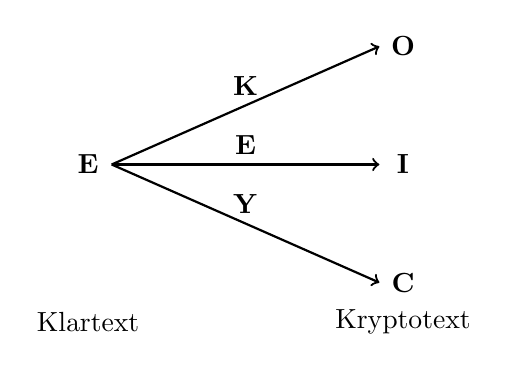
\begin{tikzpicture}
			% Klartext und Kryptotext Labels
			\node at (0, 0) {\textbf{E}};
			\node at (4, 1.5) {\textbf{O}};
			\node at (4, 0) {\textbf{I}};
			\node at (4, -1.5) {\textbf{C}};

			% Verbindungspfeile mit Schlüsseln
			\draw[->, thick] (0.3, 0) -- (3.7, 1.5) node[midway, above] {\textbf{K}};
			\draw[->, thick] (0.3, 0) -- (3.7, 0) node[midway, above] {\textbf{E}};
			\draw[->, thick] (0.3, 0) -- (3.7, -1.5) node[midway, above] {\textbf{Y}};

			% Labels Klartext und Kryptotext
			\node[align=center] at (0, -2) {Klartext};
			\node[align=center] at (4, -2) {Kryptotext};
		\end{tikzpicture}
	\end{subfigure}
	\begin{subfigure}{.45\textwidth}
		\centering
		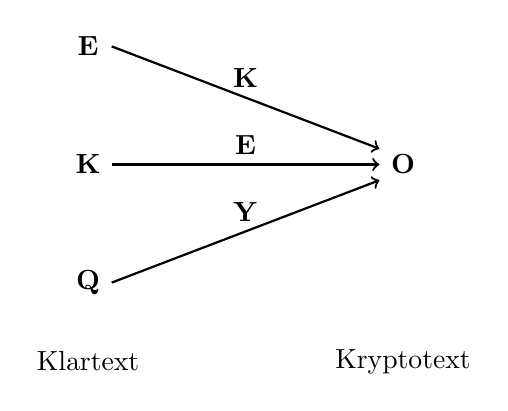
\begin{tikzpicture}
			% Klartext letters
			\node at (0, 1.5) {\textbf{E}};
			\node at (0, 0) {\textbf{K}};
			\node at (0, -1.5) {\textbf{Q}};

			% Kryptotext letter
			\node at (4, 0) {\textbf{O}};

			% Verbindungspfeile mit Schlüsseln
			\draw[->, thick] (0.3, 1.5) -- (3.7, 0.2) node[midway, above] {\textbf{K}};
			\draw[->, thick] (0.3, 0) -- (3.7, 0) node[midway, above] {\textbf{E}};
			\draw[->, thick] (0.3, -1.5) -- (3.7, -0.2) node[midway, above] {\textbf{Y}};

			% Labels Klartext und Kryptotext
			\node[align=center] at (0, -2.5) {Klartext};
			\node[align=center] at (4, -2.5) {Kryptotext};
		\end{tikzpicture}
	\end{subfigure}
	\caption{Verschlüsselungs-Möglichkeiten mit Vigenère, mit dem Schlüssel \texttt{KEY}}
	\label{fig:ex-vigenere-e}
\end{figure}
\end{mydefinition}

\begin{myremark}[Caesar ist ein Spezialfall von Vigenère]
Im Vergleich zum Verfahren von Vigenère, wird bei Caesar aus einem Buchstaben im Klartext immer derselbe Buchstabe im Kryptotext. 
Verwenden wir beispielsweise den Caesar-Schlüssel \texttt{K} (also eine Verschiebung von 10), so würde sich folgende Verschlüsselung ergeben:
\begin{verbatim}
  Klartext: I|N|F|O|R|M|A|T|I|K|I|S|T|S|O|W|A|S|V|O|N|I|N|T|E|R|E|S|S|A|N|T
 Schlüssel: K|K|K|K|K|K|K|K|K|K|K|K|K|K|K|K|K|K|K|K|K|K|K|K|K|K|K|K|K|K|K|K
Kryptotext: S|X|P|Y|B|W|K|D|S|U|S|C|D|C|Y|G|K|C|F|Y|X|S|X|D|O|B|O|C|C|K|X|D
\end{verbatim}
Aus dem Buchstaben \texttt{I} im Klartext wird also stets der Buchstabe \texttt{S} im Kryptotext, unabhängig von seiner Position relativ zum Schlüssel.

\par
Offensichtlich ist Caesar ein Spezialfall von Vigenère, bei dem der Schlüssel (das Wort) aus exakt einem einzigen Buchstaben besteht.
\end{myremark}

\begin{myexercise}\label{myexercise:vigenere-keys}
	Welche Eigenschaft muss ein Vigenère-Schlüssel haben, damit (zumindest theoretisch) aus einem Buchstaben im Klartext exakt 10 verschiedene Buchstaben im Kryptotext werden können? Geben Sie ein Beispiel für einen solchen Schlüssel an.
	\begin{myanswer}
		Der Schlüssel muss exakt 10 verschiedene Buchstaben enthalten, damit aus einem Buchstaben im Klartext 10 verschiedene Buchstaben im Kryptotext werden können. Ein Beispiel für einen solchen Schlüssel ist \texttt{ABCDEFGHIJ} oder auch \mbox{\texttt{ABCDEFGHIJABFBE}}. Damit aus einem Buchstaben $\alpha$ im Klartext genau 10 verschiedene Buchstaben im Kryptotext entstehen, müssen der Klartext und der Schlüssel so beschaffen sein, dass jeder der 10 verschiedenen Buchstaben des Schlüssels mindestens einmal mit $\alpha$ im Klartext korrespondiert (unter dem Buchstaben $\alpha$ zu stehen kommt).
	\end{myanswer}
\end{myexercise}

Das Verfahren von Vigenère galt während mehreren Jahrhunderten als sicher und wurde in zahlreichen vielen militärischen Anwendungen eingesetzt!

\subsection{Vigenère-Tabelle und praktische Umsetzung}
Wie bereits in \cref{mydefinition:vigenere} angesprochen, definiert jeder Buchstabe eines Vigenère-Schlüssels eine bestimmte Caesar-Verschiebung. 
Es ist daher sinnvoll, eine Tabelle zu erstellen, welche jede der 26 möglichen Caesar-Verschiebungen auf einen Blick darstellt. 
Diese Tabelle wird als \textbf{Vigenère-Tabelle} bezeichnet und ist in \cref{tab:vigenere} gegeben. 
Jede der 26 Spalten der Vigenère-Tabelle entspricht einer möglichen Caesar-Verschiebung (Einstellung der Caesar-Drehscheibe), welche durch den entsprechenden Schlüsselbuchstaben definiert ist.
\begin{table}[H]
    \centering
    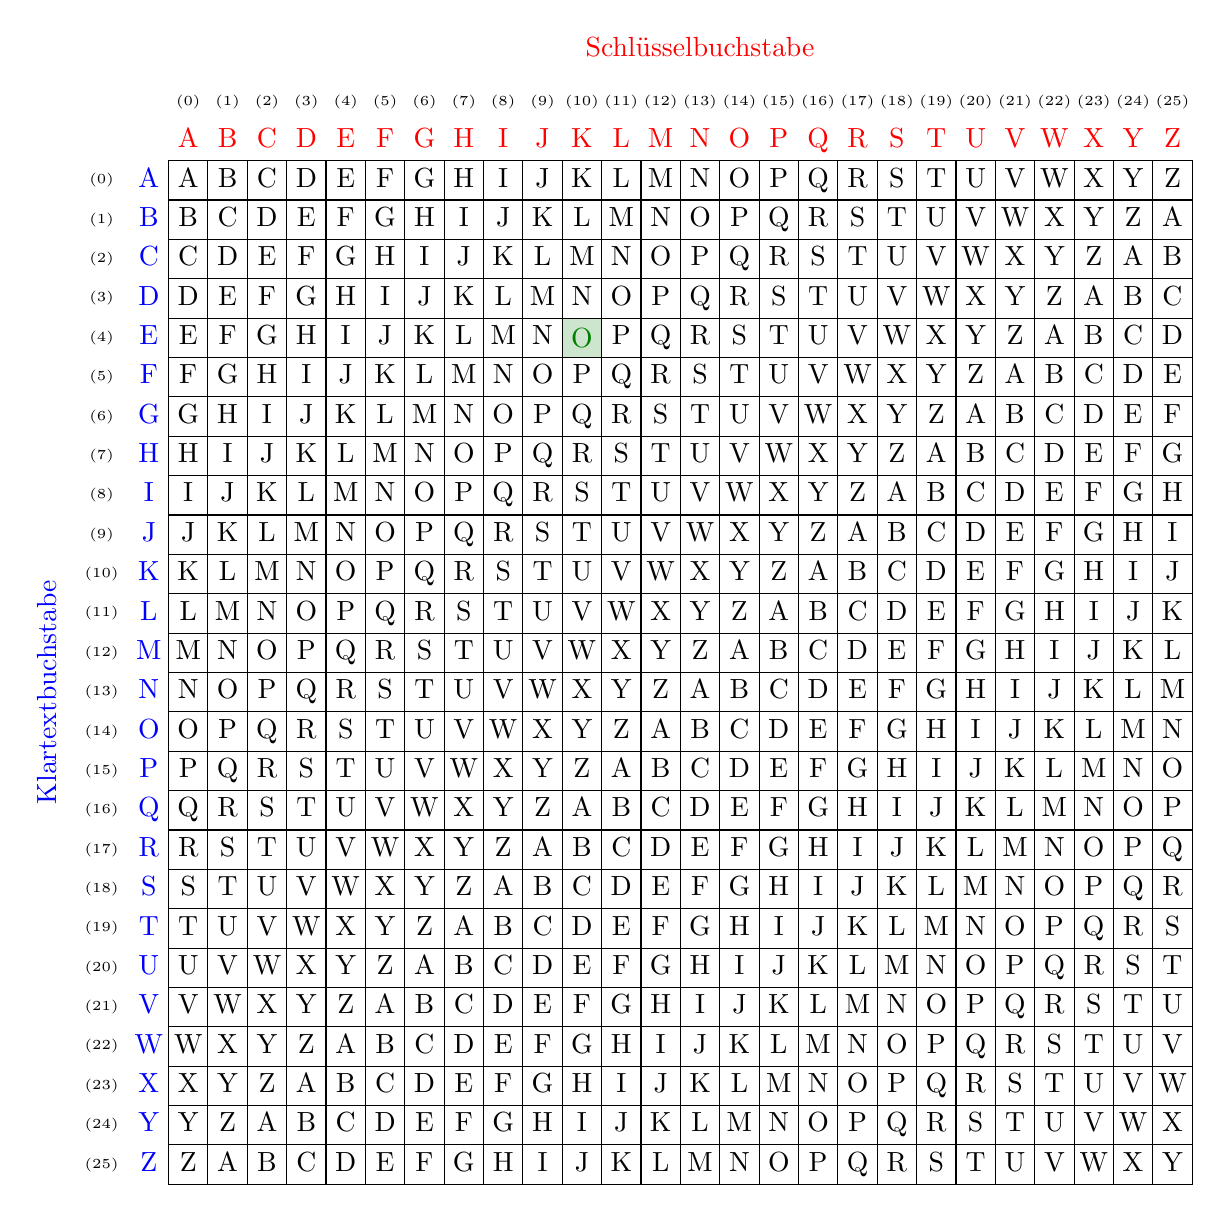
\begin{tikzpicture}
        \foreach \i in {0,...,25} {
                % Blaue Klartextbuchstaben (links) mit Ordnung davor
                \node at (-1.1,-\i*0.5) {\tiny (\i)}; % Ordnung links
                \node at (-0.5,-\i*0.5) {\textcolor{Blue}{\strut\symbol{\numexpr`A+\i\relax}}};
                
                % Rote Schlüsselbuchstaben (oben) mit Ordnung darüber
                \node at (\i*0.5,1.0) {\tiny (\i)}; % Ordnung oben
                \node at (\i*0.5,0.5) {\textcolor{Red}{\strut\symbol{\numexpr`A+\i\relax}}};
                
                \foreach \j in {0,...,25} {
                        \edef\k{\ifnum\numexpr\i+\j\relax>25
                                \the\numexpr\i+\j-26\relax
                            \else
                                \the\numexpr\i+\j\relax
                            \fi}
                        \node[draw,minimum size=0.5cm,inner sep=0pt]
                        at (\i*0.5,-\j*0.5) {\strut\symbol{\numexpr`A+\k\relax}};
                    }
            }
        
        % Markiertes Beispiel (hier angepasst auf den Buchstaben 'O')
        \node[draw,minimum size=0.5cm,inner sep=0pt,fill=Green!20] at (5.0,-2.0) {\textcolor{Green}{O}};
        
        % Beschriftungen etwas weiter nach außen geschoben, damit sie nicht mit den Zahlen kollidieren
        \node at (6.5,1.7) {\textcolor{Red}{Schlüsselbuchstabe}};
        \node[rotate = 90] at (-1.8,-6.5)  {\textcolor{Blue}{Klartextbuchstabe}};
    \end{tikzpicture}
    \caption{Vigenère-Tabelle mit numerischer Ordnung}
    \label{tab:vigenere}
\end{table}

\begin{description}
	\item[Verschlüsselung:] Soll beispielsweise der Klartextbuchstabe \texttt{E} mit dem Schlüsselteil \texttt{K} verschlüsselt werden, so findet man in der Tabelle den entsprechenden Kryptotextbuchstaben \texttt{O}.
	\item[Entschlüsselung:] Soll beispielsweise der Kryptotextbuchstabe \texttt{O} mit dem Schlüsselteil \texttt{K} entschlüsselt werden, so sucht man in der Tabelle nach dem Klartextbuchstaben, der mit \texttt{O} und \texttt{K} korrespondiert. Dies ist in diesem Fall der Buchstabe \texttt{E}.
\end{description}

\begin{myexercise}
	\textbf{Verschlüsseln} Sie folgenden Text von Hand, mit dem Schlüssel \textcolor{red}{\texttt{YES}} und mit der Methode von Vigenère:
	\begin{center}
	\textcolor{blue}{\texttt{NIEMANDKANNDASLESEN}}
	\end{center}
	\begin{myanswer}
		\texttt{LMWKEFBOSLRVYWDCWWL}
	\end{myanswer}
\end{myexercise}

\begin{myexercise}
	\textbf{Entschlüsseln} Sie folgenden Text von Hand, wenn Sie wissen, dass er mit dem Schlüssel \textcolor{red}{\texttt{TOP}} und mit der Methode von Vigenère verschlüsselt worden ist:
	\begin{center}
	\texttt{UFPOCVNHVXAPVVI}
	\end{center}
	\begin{myanswer}
		\textcolor{blue}{\texttt{BRAVOGUTGEMACHT}}
	\end{myanswer}
\end{myexercise}

Wir haben einen langen Klartext verwendet und diesen einmal mit Caesar (Schlüssel \texttt{C}, also Verschiebung 2)und einmal mit Vigenère (Schlüssel \texttt{ABCDEFG}) verschlüsselt und schliesslich die relativen Häufigkeit aller verschiedenen Buchstaben im Kryptotext in \cref{fig:langer-text-vig-caesar} dargestellt. Die relative Häufigkeit eines Buchstabens im Kryptotext ist definiert als die Anzahl der Vorkommen dieses Buchstabens geteilt durch die Gesamtanzahl aller Buchstaben im Kryptotext

\begin{figure}[H]
	\centering
	\begin{subfigure}{.49\linewidth}
		\centering
		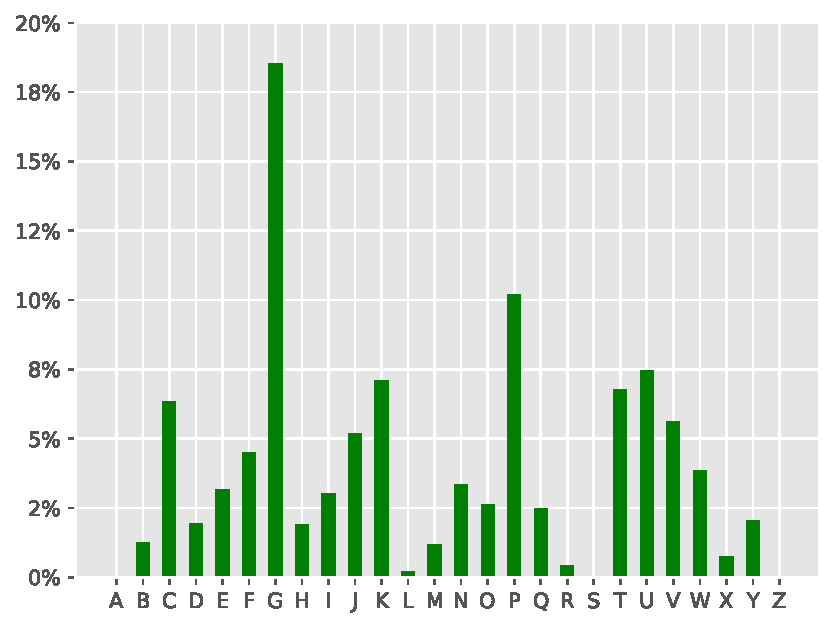
\includegraphics[width=\linewidth]{Grundlagen_Info/03_Kryptologie/Figures/caesar-freq}
		\caption{Caesar}
	\end{subfigure}
	\begin{subfigure}{.49\linewidth}
		\centering
		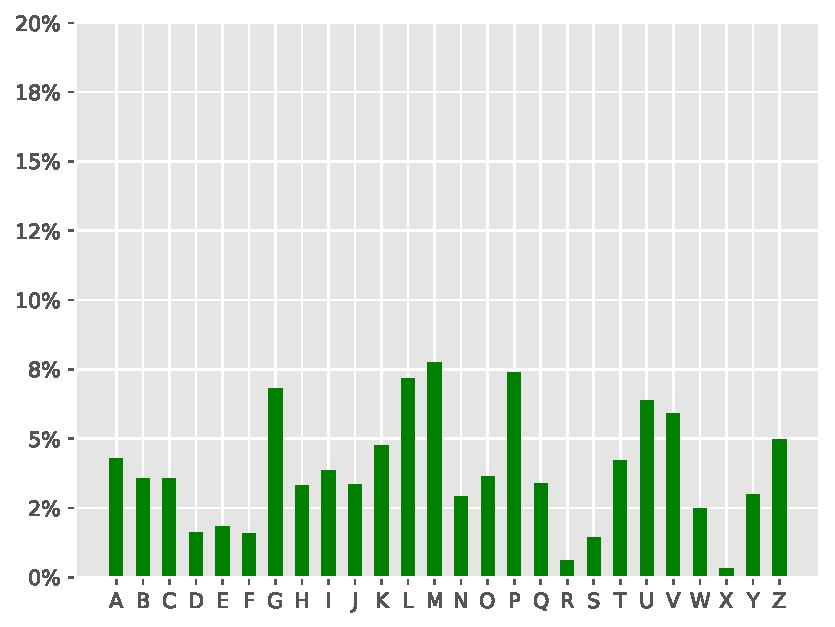
\includegraphics[width=\linewidth]{Grundlagen_Info/03_Kryptologie/Figures/vigenere-freq}
		\caption{Vigenère}

	\end{subfigure}
	\caption{relative Häufigkeit der Buchstaben im Kryptotext eines langen Texts, einmal mit Caesar (Schlüssel: \texttt{C}) und einmal mit Vigenère (Schlüssel: \texttt{ABCDEFG}) verschlüsselt}
	\label{fig:langer-text-vig-caesar}
\end{figure}

\cref{fig:langer-text-vig-caesar} zeigt, dass Vigenère zu einer insgesamt homogeneren Verteilung der relativen Buchstabenhäufigkeiten im Kryptotext führt. 
Dies kommt daher, dass bei Vigenère jeder Klartextbuchstaben auf \emph{mehrere} Kryptotext-Buchstaben verteilt wird, währenddem bei Caesar jeder Klartextbuchstaben stets auf denselben Kryptotextbuchstaben abgebildet wird.

\subsection{Kryptoanalyse von Vigenère}\label{subsubsec:vigHack}

\subsubsection{Kryptoanalyse von Vigenère bei bekannter Schlüssellänge}
Wenn die Schlüssellänge eines mit Vigenère verschlüsselten Texts bekannt ist, kann man den Klartext relativ einfach herausfinden. 
Das Vorgehen ist exemplarisch in \cref{myexample:vigHaufigkeitGruppen} beschrieben.

\begin{myexample}[Häufigkeitsanalyse von Vigenère bei bekannter Schlüssellänge]\label{myexample:vigHaufigkeitGruppen}
Angenommen, wir wüssten, dass folgender Kyrptotext durch die Verwendung eines  Vigenère-Schlüssels der Länge 3 entstanden ist:

\texttt{\colorstring[ForestGreen,RoyalBlue,Crimson]{MKUMYBVFLZDHZGOMKAMTRMKAPCAUGPVGNIPGMULMNLMKUOGUWOTMPNTGPKJKMPZCGZAGUNTBMJSQPNAOVZILVFPMKJPOPBIHVBLUJLZBLVILVKLAULQEOJKUINSMKUCPKNTLCGTQEOUGPVGZTGIMPZQPKQGZMTNMILVFKQGMCGYAQSKJLAGLTGUOGZKJHNHLVKZBYPMFPMOLQPLQEOJKUAQNTWLKMSQEOUGPVDLAVLZUVOCUHKULGTOGMCGOTGCWPYCJPOGTLCZMKUDGYAWUSGULCZAOLQPLSWUAVKITBVVLZNLQFLBKJPMVMPUBGQMVGBPPKJAHGPKJUMPUQEOBGPVGUAVYQEOCPKJKUVKLMKUOTVMUZMTLZOHTGYOGDMULVCSAKULKLAGUIWNMPITKJSGUEGUVFHANPMDL}}

Alle grünen Buchstaben entstanden durch eine Verschiebung entsprechende dem ersten Buchstaben des Vigenère-Schlüssels, alle blauen Buchstaben durch eine Verschiebung entsprechend dem zweiten Buchstaben des Vigenère-Schlüssels und alle roten Buchstaben durch eine Verschiebung entsprechend dem dritten Buchstaben des Vigenère-Schlüssels.

\par
Wenn wir die grünen, blauen und roten blauen Buchstaben jeweils zu einem eigenen Kyrptotext zusammenfassen, erhalten wir drei verschiedene Kryptotexte, welche jeweils durch eine Caesar-Verschiebung entstanden.
Damit können wir die auf jede der drei Gruppen (grün, blau, rot) die Häufigkeitsanalyse (genau analog zu \cref{sec:kryptoanalyse_caesar}) anwenden, um innerhalb der jeweiligen Gruppe die Verschiebung zu erraten, welche durch den entsprechenden Vigenère-Schlüsselbuchstaben definiert ist.

\par
In \cref{fig:vig-subgroup}) sind die relativen Häufigkeiten der Buchstaben für jede der drei Gruppen dargestellt.

\begin{figure}[H]
	\centering
\foreach \n / \name in {1/grüne, 2/blaue, 3/rote}{
    \begin{subfigure}{.3\linewidth}
        \centering
        % \n sorgt für ...group1, ...group2, ...group3
        \includegraphics[width=\linewidth]{Grundlagen_Info/03_Kryptologie/Figures/vigenere-len3-group\n}
        % \name sorgt für die korrekte Caption
        \caption{\name{}-Gruppe}
    \end{subfigure}
}
	\caption{relative Buchstabenhäufigkeit in einem durch Vigenère verschlüsselten Text pro Gruppe}
	\label{fig:vig-subgroup}
\end{figure}
Dabei erkennen wir, dass die häufigsten Buchstaben pro Gruppe \textcolor{ForestGreen}{\texttt{M}}, \textcolor{RoyalBlue}{\texttt{G}}, bzw. \textcolor{Crimson}{\texttt{L}} sind.
Da \texttt{E} der häufigste Buchstabe im Deutschen ist, können wir annehmen, dass die häufigsten Buchstaben \textcolor{ForestGreen}{\texttt{M}}, \textcolor{RoyalBlue}{\texttt{G}}, bzw. \textcolor{Crimson}{\texttt{L}} jeweils aus \texttt{E} im Klartext entstanden sind.
Dies entspricht den folgenden drei Caesar-Verschiebungen: \texttt{E}\rightarrow\texttt{M} entspricht einer Verschiebung von 8 (um \texttt{I}), \texttt{E}\rightarrow\texttt{G} einer Verschiebung von 2 (um \texttt{C}) und \texttt{E}\rightarrow\texttt{L} einer Verschiebung von 7 (um \texttt{H}).:
\begin{figure}[H]
	\centering
	\resizebox{.65\textwidth}{!}{\caesar[8] \caesar[2] \caesar[7]}
\end{figure}
Der Vigenère-Schlüssel wird also vermutlich \texttt{ICH} lauten, da $\text{ord}(\texttt{I}) = 8$, $\text{ord}(\texttt{C}) = 2$ und $\text{ord}(\texttt{H}) = 7$.
\end{myexample}

\begin{myexercise}
	Kopieren Sie den folgenden Kryptotext und versuchen Sie, ihn mit dem \href{https://cryptbreaker.marcwidmer.xyz/solve}{Analysetool} zu entziffern, wenn Sie wissen, dass die Schlüssellänge drei ist. Schauen Sie sich die Buchstabenhäufigkeiten für jede der 3 Gruppen an, indem Sie unter \emph{Analysewerkzeug} die Häufigkeitsanalyse auswählen und \emph{stride} (Schrittgrösse) 3. Unterhalb der Grafiken kann man zwischen jeder der drei Gruppen hin- und herwechseln. Probieren Sie den wahrscheinlichsten Schlüssel aus, indem Sie beim \emph{Entschlüsselungswerkzeug} die Methode \emph{Vigenère} auswählen und den Schlüssel eingeben.

	\texttt{\colorstring[black]{WORBHHHLUQOWWLDSYSQOWOUKSUDSNEGAAZAEBKISMRILHGPCVLIBZTRLMHYUSIEBILWJKULZSPGHCEFZUQOIQOWCOLSBCVKISZMOSFSZTNBHOSTSUFILHZPCVTEWUHSYZBVCVQEBLMKHHBNEBLIUAIVYDFHEBNTSBCVGUBBNUBTGVMCLGHPHFDAZAEBDISPHFHUGKUBZTIUDBLBSSUATIQOSHLIUAMSPNPBS}}

	\begin{myanswer}
		Mit dem Schlüssel \texttt{OHA} kommen wir auf folgende Lösung:

		\texttt{\colorstring[black]{IHRNAHTEUCHWIEDERSCHWANKENDEGESTALTENDIEFRUEHSICHEINSTDEMTRUEBENBLICKGEZEIGTVERSUCHICHWOHLEUCHDIESMALFESTZUHALTENFUEHLICHMEINHERZNOCHJENEMWAHNGENEIGTIHRDRAENGTEUCHZUNUNGUTSOMOEGTIHRWALTENWIEIHRAUSDUNSTUNDNEBELUMMICHSTEIGTMEINBUS}}
	\end{myanswer}
\end{myexercise}
\begin{minipage}{\textwidth} % wrapping this exercise in a minipage to enable printing it out on one page
	\begin{myexercise}[Vigenère knacken bei bekannter Schlüssellänge (zu dritt)]\label{ex:vigHaufigkeitGruppen}

		Finden Sie für folgenden Vigenère-Text den Klartext heraus, wenn Sie wissen, dass der Schlüssel Länge 3 hat:

		\colorstring[ForestGreen,RoyalBlue,Crimson]{WKJLMUAKJWZJWQVWVVKBGZBGJAVOMPFRGVMTWZMWVPLEKWMNWUGFBCJMKFMXWZNSMUKTKUPGNMTKKJDCGKAGDCPYNWWZWFAGJMHJMKZMKLQUL}

		\begin{enumerate}
			\item Finden Sie zuerst die häufigsten Buchstaben pro Gruppe heraus (Gruppe 3 ist bereits gemacht, s. unten). Seien Sie genau, ansonsten müssen Sie später wieder von vorne beginnen!
			      \notiz{4}
			\item Finden Sie danach den Schlüssel heraus, indem Sie annehmen, dass der häufigste Buchstabe im Geheimtext den Buchstaben \texttt{E} im Klartext repräsentiert. Für Gruppe 3 ist die Lösung bereits vorgegeben.
			      \begin{table}[H]
				      \centering
				      \begin{tabular}{c||c|c}
					                                                 & \textbf{Häufigster Buchstabe} & \textbf{Schlüssel}                               \\\midrule\midrule
					      \textbf{\textcolor{ForestGreen}{Gruppe 1}} &                               &                                                  \\\midrule
					      \textbf{\textcolor{RoyalBlue}{Gruppe 2}}   &                               &                                                  \\\midrule
					      \textbf{\textcolor{Crimson}{Gruppe 3}}     & \texttt{(E $\rightarrow$) G}  & \texttt{(A $\rightarrow$) C} (=2 Verschiebungen) \\
				      \end{tabular}
			      \end{table}
			\item Entschlüsseln Sie nun den Geheimtext, indem Sie die \href{https://inventwithpython.com/cipherwheel/}{Caesar-Drehscheiben} verwenden (Tipp: Machen Sie jeweils eine Farbgruppe pro Mal).
		\end{enumerate}

		\colorstringunderline[ForestGreen,RoyalBlue,Crimson]{ECHTESICHERHEITENTSTEHTERSTWENNJEDERERKENNTWIEELEMENTAREINEVERLAESSLICHEVERSCHLUESSELUNGFUERUNSEREFREIHEITIST}


		\begin{myanswer}
			\begin{table}[H]
				\centering
				\begin{tabular}{c||c|c}
					                                           & \textbf{Häufigster Buchstabe} & \textbf{Schlüssel}                                \\\midrule\midrule
					\textbf{\textcolor{ForestGreen}{Gruppe 1}} & \texttt{(E $\rightarrow$) W}  & \texttt{(A $\rightarrow$) S} (=18 Verschiebungen) \\\midrule
					\textbf{\textcolor{RoyalBlue}{Gruppe 2}}   & \texttt{(E $\rightarrow$) M}  & \texttt{(A $\rightarrow$) I} (=8 Verschiebungen)  \\\midrule
					\textbf{\textcolor{Crimson}{Gruppe 3}}     & \texttt{(E $\rightarrow$) G}  & \texttt{(A $\rightarrow$) C} (=2 Verschiebungen)  \\
				\end{tabular}
			\end{table}

			\colorstring[ForestGreen,RoyalBlue,Crimson]{ECHTESICHERHEITENTSTEHTERSTWENNJEDERERKENNTWIEELEMENTAREINEVERLAESSLICHEVERSCHLUESSELUNGFUERUNSEREFREIHEITIST}
		\end{myanswer}
	\end{myexercise}
\end{minipage}


\subsubsection{Bestimmung der Schlüssellänge mit dem Kasiski-Test}
Wie Sie gesehen haben, kann man Vigenère \emph{gruppenweise} mit denselben Methoden knacken, die wir benutzt haben, um Caesar zu knacken. Falls die Schlüssellänge unbekannt ist, können sowohl der Kasiski-Test wie auch die Friedmansche Charakteristik verwendet werden, um diese zu erraten. In diesem Unterabschnitt schauen wir uns zunächst den Kasiski-Test an.

Friedrich Kasiski war ein preussischer Infanteriemajor (1805 - 1881), welcher mit seinem Kasiski-Test massgeblich zum Knacken der Vigenère-Verschlüsselung beigetragen hat. Den Kasiski-Test veröffentlichte er 1863 in seinem Buch \enquote{Die Geheimschriften und die Dechiffrir-Kunst} (siehe \cref{fig:kasiski-test-book}).

\begin{figure}[H]
	\centering
	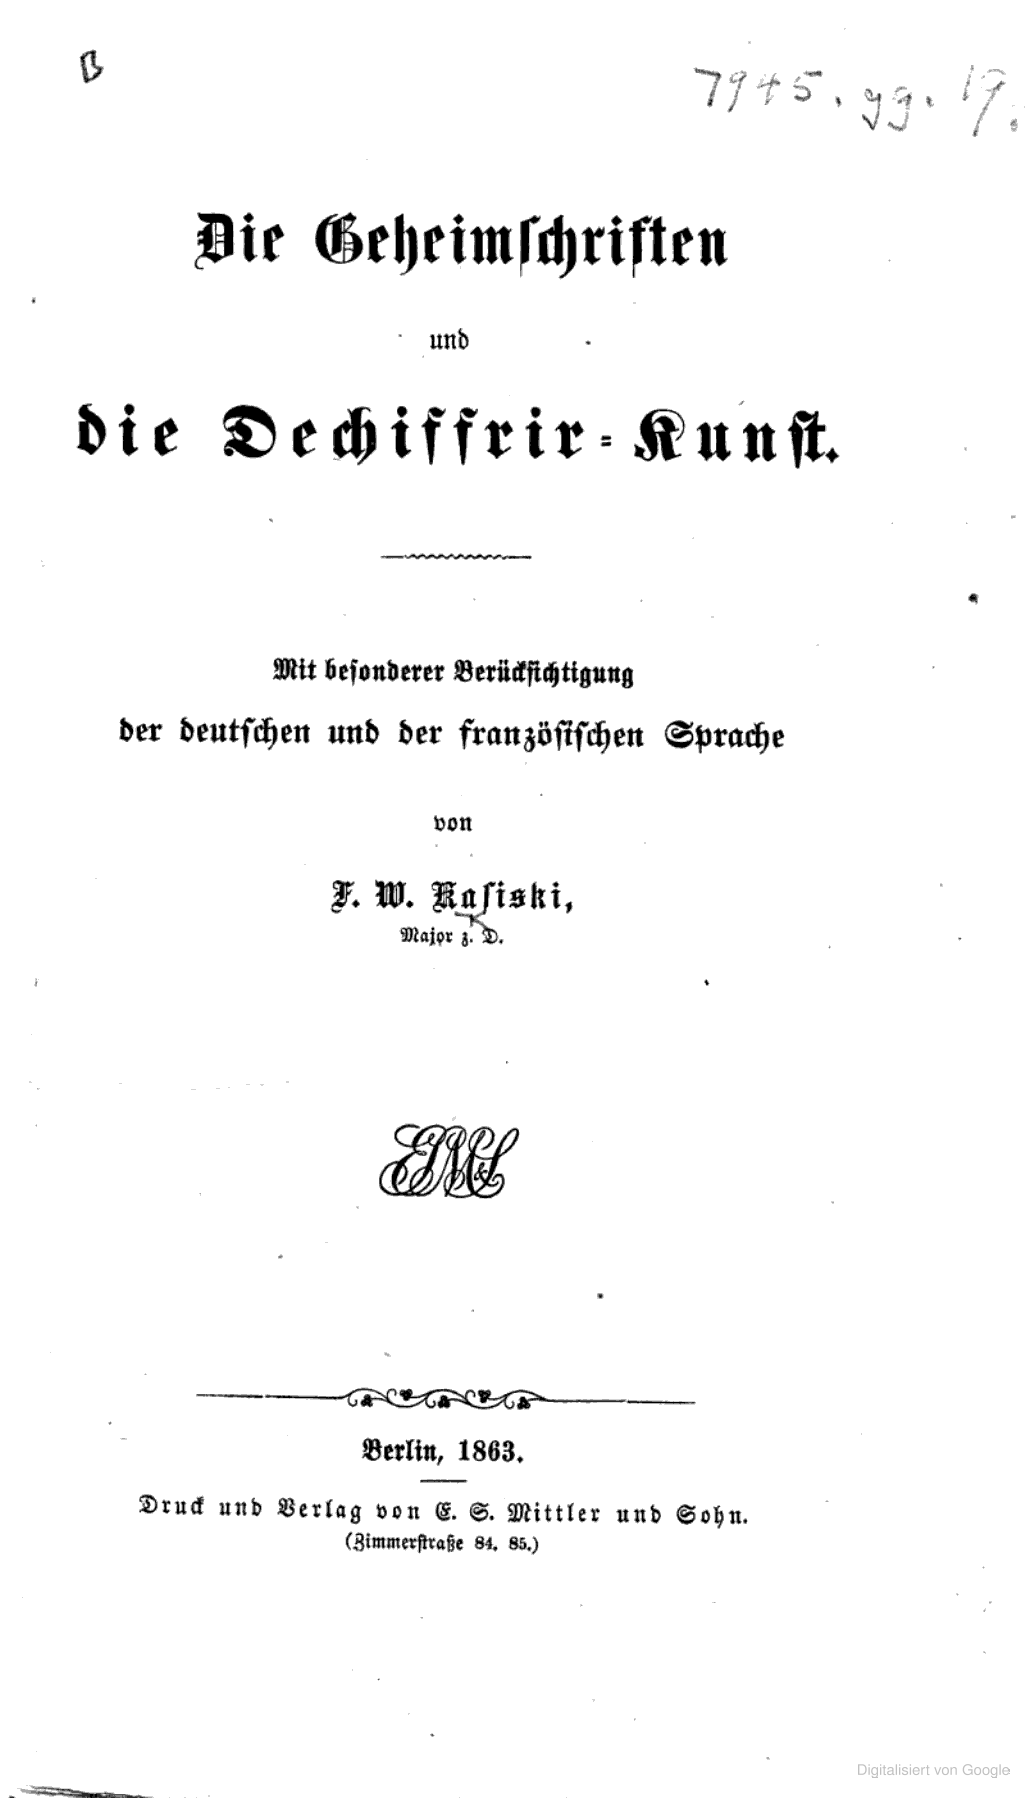
\includegraphics[width=.4\linewidth]{Grundlagen_Info/03_Kryptologie/Figures/kasiski-book}
	\caption{Umschlag des Buches \enquote{Die Geheimschriften und die Dechiffrir-Kunst} von Friedrich Kasiski (1863, \href{https://books.google.de/books?id=fB5dAAAAcAAJ}{Quelle})}
	\label{fig:kasiski-test-book}
\end{figure}

Die Grundidee hinter dem Kasiski-Test ist: Wenn ein Wort oder ein Wortteil im Klartext mehrmals vorkommen, so wird dieser möglicherweise auch im Kryptotext mehrmals vorkommen. Wenn beispielsweise die Buchstaben \texttt{DIE} mehrmals mit dem Schlüssel \texttt{KEY} verschlüsselt werden, dann wird der Text \texttt{LIV} mehrmals im Geheimtext auftauchen. Wenn das Wort \texttt{DIE} also zweimal im Klartext vorkommt \textbf{und} auf denselben Schlüsselteil (\texttt{KEY}, \texttt{EYK} oder \texttt{YKE}) fällt, wird z.B. \texttt{LIV} auch zweimal im Kryptotext gleich verschlüsselt sein.

Wenn wir also im Kryptotext nach wiederholten Sequenzen suchen, können wir daraus die Schlüssellänge ableiten.

\begin{myexample}\label{ex:kasiskiTest}
In folgendem Beispiel ist der Klartext auf der ersten Zeile. Der Schlüssel \texttt{CODE} wird verwendet, um den Geheimtext (auf der dritten Zeile) zu erzeugen:

\texttt{M\gold{EIN}KL\red{EIN}ERREIMSCH\red{EIN}TK\green{EIN}ERZUS\green{EIN}}

\texttt{C\gold{ODE}CO\red{DEC}ODECODECO\red{DEC}OD\green{ECO}DECOD\green{ECO}}

\texttt{O\annotKasiski{Gold}{S}{LR}{2}MZ\annotKasiski{red}{H}{MP}{7}SUVGWPWEV\annotKasiski{red}{H}{MP}{19}HN\annotKasiski{ForestGreen}{I}{KB}{24}HVBIV\annotKasiski{ForestGreen}{I}{KB}{32}\\[.5cm]}

% OSLRMZHMPSUVGWPWEVHMPHNIKBHVBIVIKB


Der Kasiski-Test erlaubt uns, Hinweise auf die Schlüssellänge zu erhalten, ohne den Schlüssel zu kennen:
\begin{itemize}
	\item Die Sequenzen \texttt{HMP} und \texttt{IKB} erscheinen je zweimal im Geheimtext.
	\item Die Sequenz \texttt{HMP} befindet sich an den Positionen 7 und 19. Die Differenz zwischen diesen Positionen beträgt 12. Wenn beide \texttt{HMP} das gleiche Trigramm kodieren (in diesem Fall das Trigramm \texttt{EIN}), muss die Schlüssellänge ein Teiler von 12 sein.
	\item Die Sequenz \texttt{IKB} befindet sich an den Positionen 24 und 32. Die Differenz zwischen diesen Positionen beträgt 8. Wenn beide \texttt{IKB} das gleiche Trigramm kodieren, muss die Schlüssellänge ein Teiler von 8 sein.
	      %   \begin{tcolorbox}
	      %       $\mathbf{\underset{\text{Position 1 \texttt{IKB}}}{8}+\underset{\text{Anzahl Codewörter}}{6}\times \underset{\text{Codewort-Länge!}}{\blue{4}} = \underset{\text{Position 2 \texttt{IKB}}}{32}}$
	      %   \end{tcolorbox}
	\item Die gemeinsamen Teiler von 24 und 8 sind 1, 2 und 4. Die Schlüssellänge muss einer dieser Teiler sein. Aus dieser Information alleine können wir die Schlüssellänge nicht eindeutig bestimmen, aber wir haben die Anzahl der Möglichkeiten bereits stark eingeschränkt. In diesem Fall ist die korrekte Schlüssellänge 4.
\end{itemize}
\end{myexample}

\clearpage  % using clearpage to enable printing out the exercise on just one page
\begin{myexercise}[Vigenère knacken bei bekannter Schlüssellänge (zu dritt)]\label{ex:vigKasiski}
	Finden Sie den Klartext für folgende Nachricht heraus, wenn Sie wissen, dass der Text mit Vigenère verschlüsselt worden ist. Wenden Sie den Kasiski-Test an!

	\begin{alltt}
		UEU\underline{I}\underline{O}\underline{O}CEU\(\underset{\makebox[\widthof{\texttt{X}}][c]{\footnotesize\texttt{\red{10}}}}{\texttt{\red{D}}}\)IW\underline{I}\underline{O}\underline{O}WRRC\(\underset{\makebox[\widthof{\texttt{X}}][c]{\footnotesize\texttt{\red{20}}}}{\texttt{\red{L}}}\)WVUQURRCL\(\underset{\makebox[\widthof{\texttt{X}}][c]{\footnotesize\texttt{\red{30}}}}{\texttt{\red{W}}}\)VNDTHXETH\(\underset{\makebox[\widthof{\texttt{X}}][c]{\footnotesize\texttt{\red{40}}}}{\texttt{\red{E}}}\)RRCFKRTWV\(\underset{\makebox[\widthof{\texttt{X}}][c]{\footnotesize\texttt{\red{50}}}}{\texttt{\red{S}}}\)FYOQRNJJT\(\underset{\makebox[\widthof{\texttt{X}}][c]{\footnotesize\texttt{\red{60}}}}{\texttt{\red{G}}}\)\\[.5cm]\rule{\linewidth}{1pt}
		RSVUAV\underline{I}\underline{O}\underline{O}\(\underset{\makebox[\widthof{\texttt{X}}][c]{\footnotesize\texttt{\red{70}}}}{\texttt{\red{C}}}\)EQEIHRUIY\(\underset{\makebox[\widthof{\texttt{X}}][c]{\footnotesize\texttt{\red{80}}}}{\texttt{\red{O}}}\)HITQLNJZN\(\underset{\makebox[\widthof{\texttt{X}}][c]{\footnotesize\texttt{\red{90}}}}{\texttt{\red{J}}}\)VSEVRJRUI\(\underset{\makebox[\widthof{\texttt{X}}][c]{\footnotesize\texttt{\red{100}}}}{\texttt{\red{L}}}\)NGUEU\underline{I}\underline{O}\underline{O}C\(\underset{\makebox[\widthof{\texttt{X}}][c]{\footnotesize\texttt{\red{110}}}}{\texttt{\red{E}}}\)UDIW\underline{I}\underline{O}\underline{O}WH\(\underset{\makebox[\widthof{\texttt{X}}][c]{\footnotesize\texttt{\red{120}}}}{\texttt{\red{R}}}\)\\[.5cm]\rule{\linewidth}{1pt}
		VRWVAXWZX\underline{\(\underset{\makebox[\widthof{\texttt{X}}][c]{\footnotesize\texttt{\red{130}}}}{\texttt{\red{I}}}\)}\underline{O}\underline{O}CEQ\underline{I}\underline{O}\underline{O}W\(\underset{\makebox[\widthof{\texttt{X}}][c]{\footnotesize\texttt{\red{140}}}}{\texttt{\red{A}}}\)WDEWVAXWU\(\underset{\makebox[\widthof{\texttt{X}}][c]{\footnotesize\texttt{\red{150}}}}{\texttt{\red{Q}}}\)UWRCLWVDL\(\underset{\makebox[\widthof{\texttt{X}}][c]{\footnotesize\texttt{\red{160}}}}{\texttt{\red{V}}}\)NDVCKJTHE\(\underset{\makebox[\widthof{\texttt{X}}][c]{\footnotesize\texttt{\red{170}}}}{\texttt{\red{T}}}\)DXEYFMUFL\(\underset{\makebox[\widthof{\texttt{X}}][c]{\footnotesize\texttt{\red{180}}}}{\texttt{\red{O}}}\)\\[.5cm]\rule{\linewidth}{1pt}
		VRQZCKKSP\(\underset{\makebox[\widthof{\texttt{X}}][c]{\footnotesize\texttt{\red{190}}}}{\texttt{\red{V}}}\)HUYOHIEQ\\[.5cm]\rule{\linewidth}{1pt}
	\end{alltt}
	\normalsize

	\textbf{Anleitung:}
	\begin{itemize}
		\item Die Position an allen 10, 20, 30 etc. Buchstaben sind oben bereits markiert, ebenso wie Vorkommnisse des Trigramms \underline{\texttt{IOO}}.
		\item Auf separatem Blatt:
		      \begin{enumerate}
			      \item Notieren Sie sich die \textbf{Anfangspositionen} aller Trigramme \underline{\texttt{IOO}}.
			      \item Berechnen Sie die \textbf{Abstände} zwischen den Anfangspositionen. Es reicht, wenn Sie nur die Abstände aller Anfangspositionen von \underline{IOO} zum ersten Trigramm \underline{IOO} an Position 4 berechnen.
			      \item Zerlegen Sie die Abstände zwischen den Trigrammen in \textbf{Primfaktoren}.
			      \item Finden Sie den \textbf{grössten gemeinsamen Teiler} dieser Primfaktoren, um die Schlüssellänge zu erraten.
		      \end{enumerate}
		\item Wenn Sie die Schlüssellänge haben, färben Sie den Text abwechslungsweise ein, wie in \cref{ex:vigHaufigkeitGruppen}. Teilen Sie sich zu dritt auf, so dass jede Person eine Gruppe von Buchstaben entschlüsselt (gleich wie in \cref{ex:vigHaufigkeitGruppen}).
		\item \textbf{Tipp}: Der letzte Teil des Schlüssels ist \texttt{D}. Der Schlüssel ergibt ein Wort. Entschlüsseln Sie den Text nun mit den \href{https://inventwithpython.com/cipherwheel/}{Caesar-Drehscheiben}! Entschlüsseln Sie zuerst nur die erste Zeile, um zu überprüfen, ob ihr Schlüssel stimmt und zu einem sinnvollen Text führt.
	\end{itemize}
	\begin{myanswer}
		Positionen der Anfangs-Trigramme: 4, 13, 67, 106, 115, 130, 136. Abstände und Primfaktoren sind beispielsweise:
		\begin{align*}
			13-4  & = & 9   & = & 3\times3                \\
			67-4  & = & 63  & = & 3\times3\times7         \\
			106-4 & = & 102 & = & 2\times3\times17        \\
			115-4 & = & 111 & = & 3\times37               \\
			130-4 & = & 126 & = & 2\times3\times3\times7  \\
			136-4 & = & 132 & = & 2\times2\times3\times11 \\
		\end{align*}

		Man erkennt, dass die Primzahl 3 bei jeder Differenz vorkommt, also ist der Schlüssel vermutlich 3. Wir können nun wie in \cref{ex:vigHaufigkeitGruppen} verfahren, um den Text zu knacken. Mittels Häufigkeitsanalyse (und etwas Ausprobieren mit dem häufigsten, zweithäufigsten Buchstaben etc.) finden wir folgenden Schlüssel heraus: \texttt{RAD}. Somit kann der Klartext nun entziffert werden:

		\colorstring[ForestGreen,RoyalBlue,Crimson]{DERROLLERMITROLFROLLTEUNDROLLTENACHUNTENROLFHATTESCHONANGSTDASSDASROLLENNIEAUFHOERTNUNGINGESBERGAUFUNDDERROLLERMITROLFHOERTEAUFZUROLLENROLFATMETEAUFUNDWOLLTEDIENAECHSTENTAGEVOMROLLERNICHTSMEHRHOEREN}
	\end{myanswer}
\end{myexercise}

\begin{myexercise}
	Finden Sie die Schlüssellänge für folgenden Vigenère-Text heraus, indem Sie den Kasiski-Test anwenden:

	\texttt{\colorstring[black]{CMFBAMXPESRGILLDMNCEDMTKEHRPVFEIOKLHGIVSJYSQZDMUXYLRBJITQNZTDMOVMUMFCSDMUZGDRTTHVISGUMOURNFICFTRMFSEQIJKESJBVHHKFLNCPFINVMMCIFIKLGDRECIBLFRUEIJEEFCNEARMBCELEULRTREUALMURUEHJVAMJPIDDVVEGDRFZNDWIFCGWDYUKWULDHYNJVNVOVBDREVRESFIDDVVEGHRUVLKILKUDPMVREEFYIFOFZTDRVEDEISKIFOFZTDRXVRCIOUIDNVXEMHMZCGIORUBLJEIGVFIPDVTFEMPJTHDRFETVMDBLTRHLNSISJTTIUQTHQWFRKMFXEMHFELDMUSIKHTZNCDJVLDYOUWDVUVFDWUXEGEMKEMRBTHCIOVNRMDYDHITTHTPBEGDLPVRHKFEIMMIIEQXBVGKMDYEMESSEHXSZCGXFEERFJCDDXALDDQEZEFVVEDKEHVFTISUIDFFIPQYFWUMKVESDVFJTTRTLNCJVVRCM}}

	Verwenden Sie dazu folgendes Online-Tool: \url{https://cryptbreaker.marcwidmer.xyz/solve}
	\begin{enumerate}
		\item Verwenden Sie das Analyse-Werkzeug \emph{Kasiski-Analyse}, um die Abstände der sich wiederholenden Sequenzen der Länge 4 zu bestimmen.
		      \begin{itemize}
			      \item Notieren Sie sich die Positionen und Abstände der sich wiederholenden Sequenzen der Länge 4.
			      \item Zerlegen Sie die Abstände in Primfaktoren.
			      \item Finden Sie den grössten gemeinsamen Teiler der Abstände, um die Schlüssellänge zu erraten.
		      \end{itemize}
		\item Überprüfen Sie Ihre Vermutung, indem Sie im Analyse-Werkzeug die Häufigkeitsanalyse mit der Schrittweite (\emph{stride}) gleich der vermuteten Schlüssellänge durchführen.
		\item Entschlüsseln Sie den Text mit dem \emph{Vigenère}-Entschlüsselungswerkzeug.
	\end{enumerate}

	\begin{myanswer}
		\begin{enumerate}
			\item Wir beobachten folgende Positionen und Abstände bei den Zeichenfolgen der Länge 4:
			      \begin{itemize}
				      \item \texttt{XEMH}: 283, 348 (Abstand 65) $\rightarrow$ $5\times13$
				      \item \texttt{IDDV}: 223, 178 (Abstand 45) $\rightarrow$ $3\times3\times5$
			      \end{itemize}
			      Bereits aus diesen beiden Zeichenfolgen erkennen wir einen gemeinsamen Teiler von 5 und somit eine mögliche Schlüssellänge von 5.
			\item Die Häufigkeitsanalyse mit Schrittweite 5 bestätigt unsere Vermutung, da die Häufigkeitsverteilung pro Gruppe stark von der Gleichverteilung abweicht.
			\item Mit dem Schlüssel \texttt{ZEBRA} können wir den Text entschlüsseln und erhalten einen Ausschnitt des \href{https://www.ksimlee.ch/schule/leitbild/}{Leitbilds der Kantonsschule im Lee}.
		\end{enumerate}
	\end{myanswer}
\end{myexercise}

\begin{myexercise}
	\begin{enumerate}
		\item Erklären Sie kurz: Dopplungen im Klartext (z.B. \texttt{EIN}) führen nicht unbedingt zu Dopplungen im Geheimtext.
		\item Erklären Sie kurz: Dopplungen im Geheimtext müssen nicht in jedem Fall aus Dopplungen im Klartext stammen; sie können auch zufällig entstehen.
	\end{enumerate}

	\begin{myanswer}
		Kurzbegründungen:
		\begin{itemize}
			\item Bei polyalphabetischer Verschlüsselung werden gleiche Trigramme an verschiedenen Textpositionen oft mit verschiedenen Schlüsselzeichen verschlüsselt, sodass Wiederholungen im Klartext nicht zwangsläufig gleiche Geheimtrigramme ergeben (s. z.B. \cref{ex:kasiskiTest}).
			\item Geheimtext-Dopplungen können aber auch zufällig entstehen (z.B. \texttt{OML}), wenn verschiedene Klartextfolgen unter unterschiedlichen Schlüsselteilen zufällig identische Geheimfolgen produzieren. Beispiel:
			      \begin{itemize}
				      \item Klartext: \texttt{EIN} mit Schlüsselteil \texttt{KEY} $\rightarrow$ Geheimtext: \texttt{OML}
				      \item Klartext: \texttt{KOB} mit Schlüsselteil \texttt{EYK} $\rightarrow$ Geheimtext: \texttt{OML}
			      \end{itemize}
		\end{itemize}
	\end{myanswer}
\end{myexercise}

\begin{mychallenge}
	Versuchen Sie, auf diesem Link eine weitere Challenge-Aufgabe zu lösen, indem Sie die Werkzeuge \emph{Kasiski}, \emph{Frequency} (Häufigkeit) und \emph{Vigenère} verwenden:

	\qrcode[height=2cm]{https://cryptbreaker.marcwidmer.xyz/problems/vigenere}
\end{mychallenge}

%% Link führt ins Leere
% \begin{mychallenge}
% 	Lösen Sie den Kasiski-Test online:
% 	\qrcode[height=2cm]{https://www.dominikus-gymnasium.de/kasiski-test-spiel.html}
% \end{mychallenge}

\subsubsection{Bestimmung der Schlüssellänge: Friedmansche Charakteristik}

Eine weitere Möglichkeit, die Schlüssellänge zu erraten, besteht in der Verwendung der sogenannten Friedmanschen Charakteristik.

William Friedman (1891-1969) war ein russisch-amerikanischer Kryptologe und Pionier auf dem Gebiet der Kryptoanalyse (siehe \cref{fig:william-friedman}). Kurz vor dem Ausbruch des zweiten Weltkriegs gründete er den Signals Intelligence Service (SIS), eine Geheimabteilung des US-Militärs zur Entzifferung feindlicher Codes und Geheimschriften.

\begin{figure}[H]
	\centering
	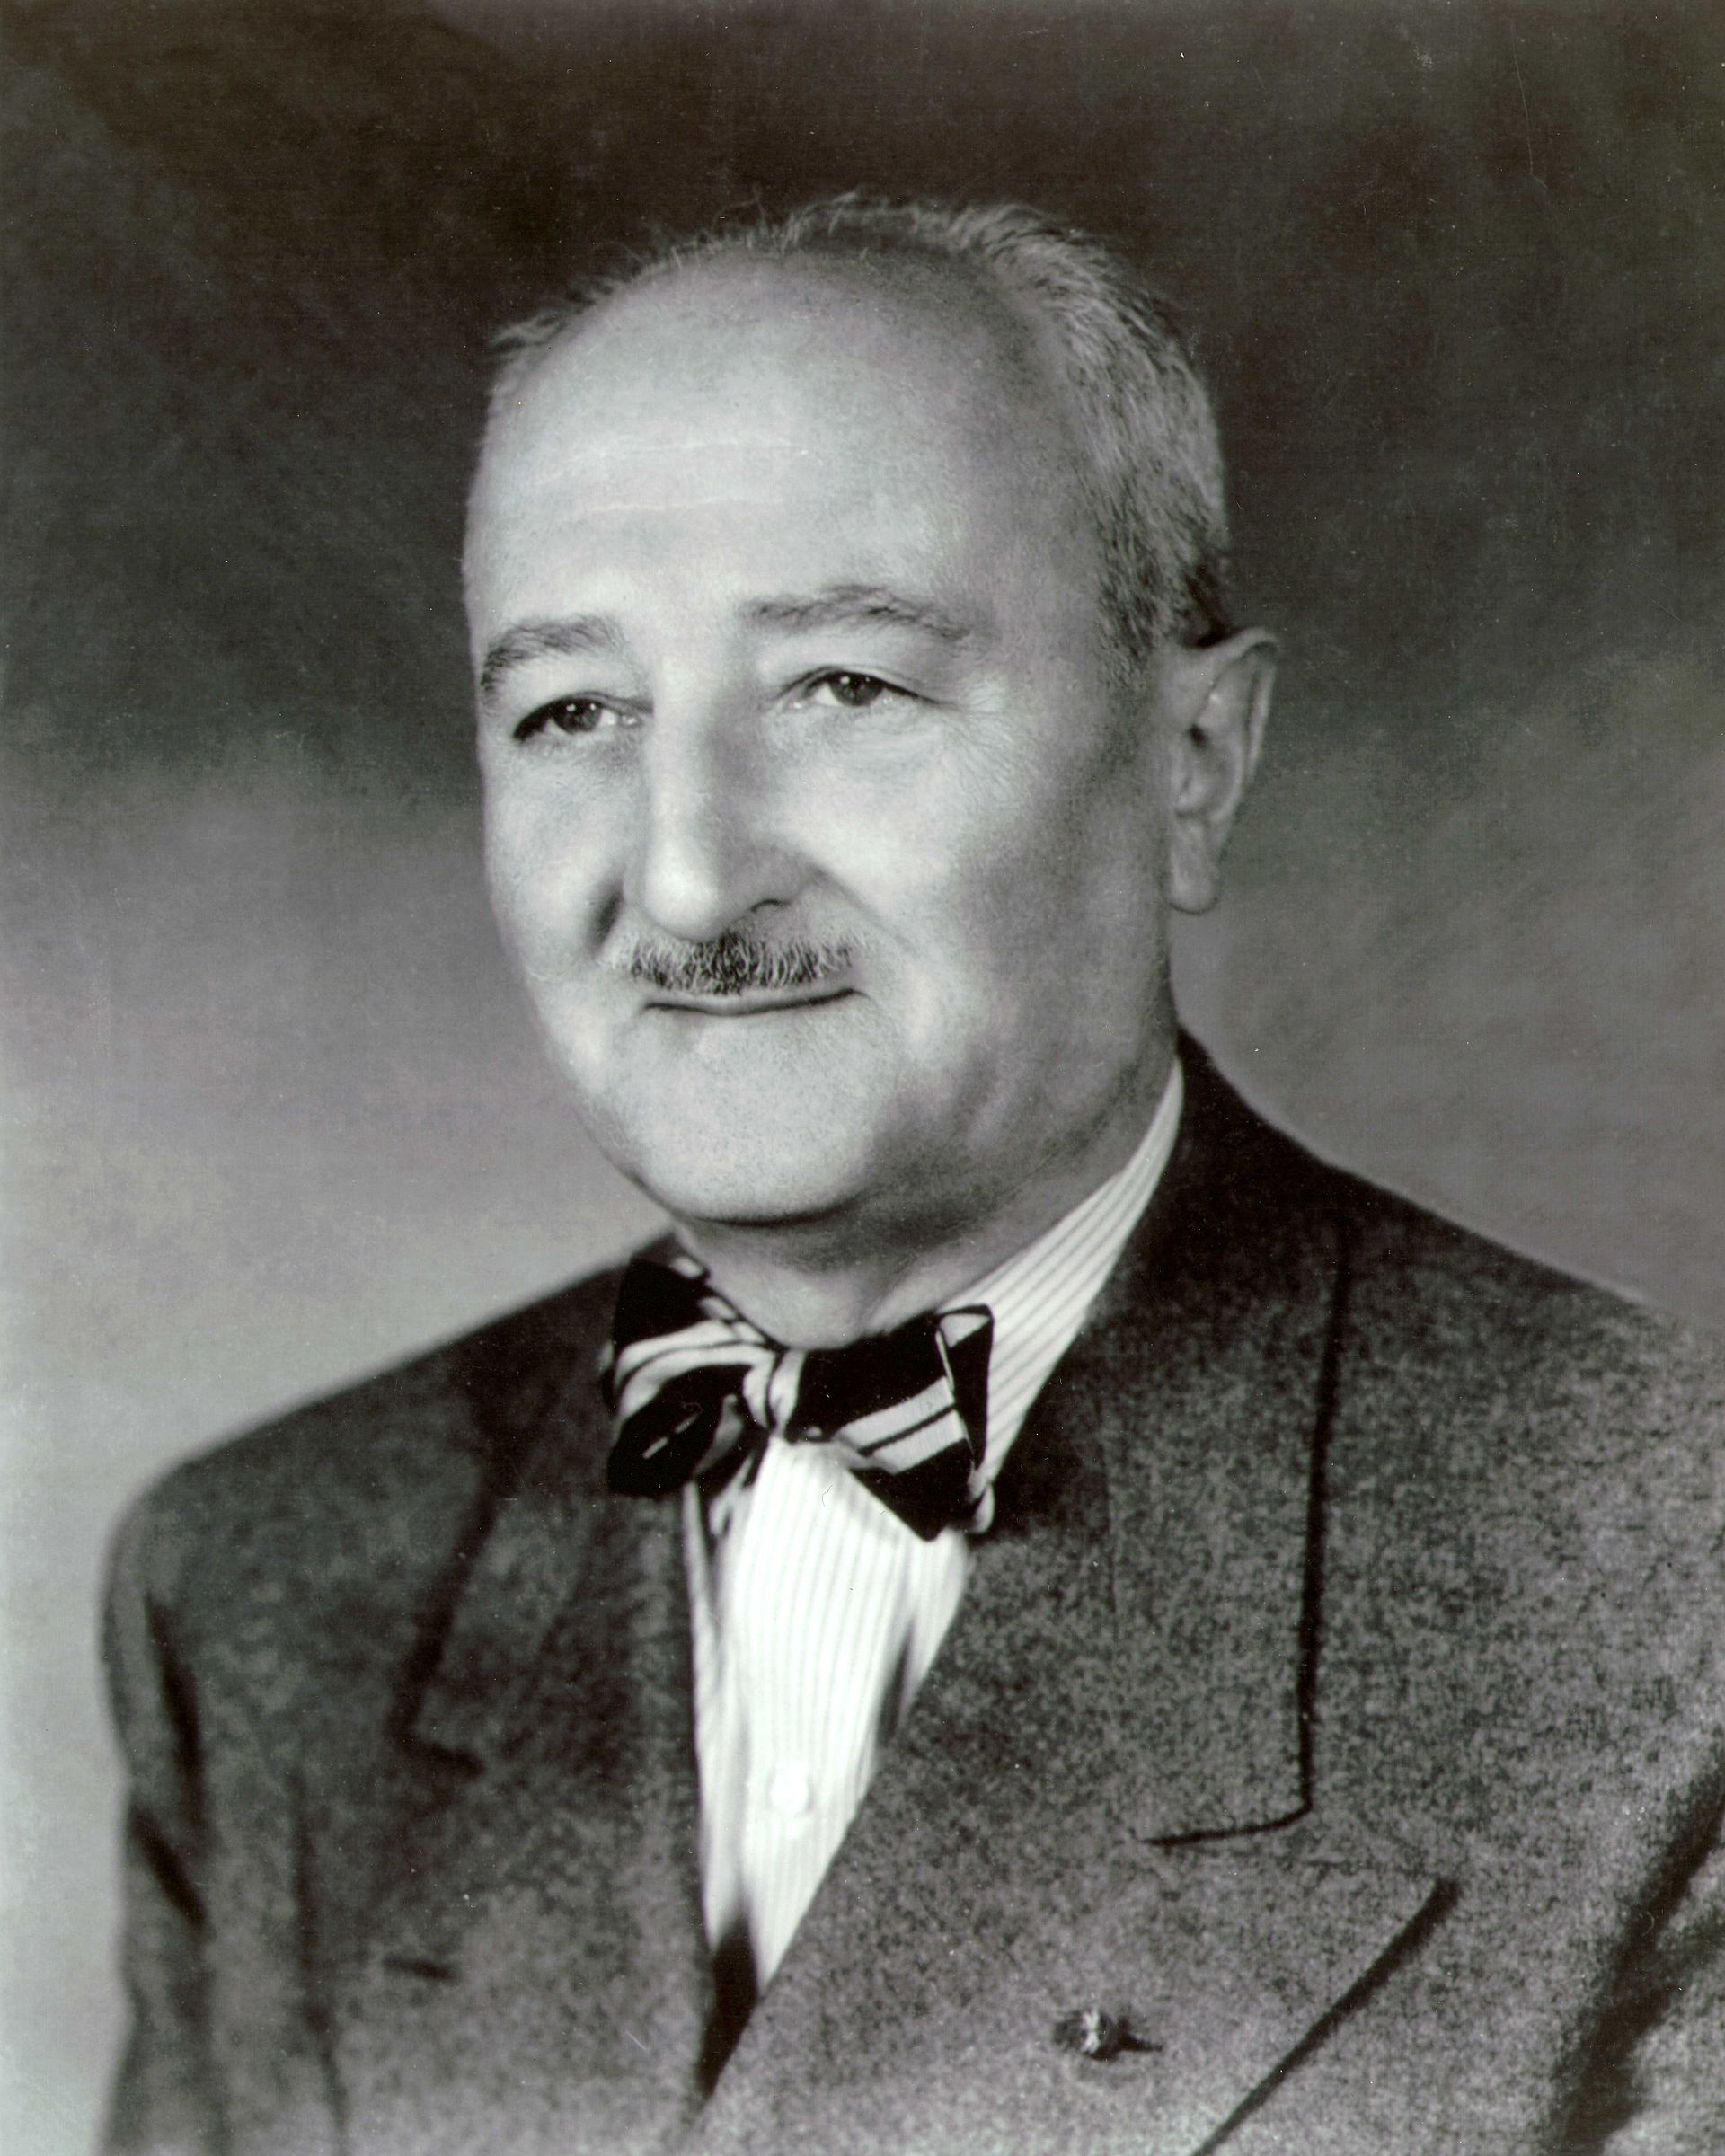
\includegraphics[width=.3\linewidth]{Grundlagen_Info/03_Kryptologie/Figures/William-Friedman.jpg}
	\caption{William Friedman (\href{https://de.wikipedia.org/wiki/William\_Friedman\#/media/Datei:William-Friedman.jpg}{Quelle})}
	\label{fig:william-friedman}
\end{figure}

Die Friedmansche Charakteristik macht sich zunutze, dass Buchstaben im Klartext ungleich verteilt sind. Falls jeder Buchstabe gleich häufig vorkommen würde, wäre die erwartete Häufigkeit jedes Buchstabens genau $1/26$. In keiner natürlichen Sprache besitzen alle Buchstaben dieselbe relative Häufigkeit. Die Häufigkeitsverteilung der Buchstaben in deutschen Texten haben wir bereits in \cref{tab:alle-haeufigkeiten} gesehen. Die relative Häufigkeit des Buchstabens \texttt{E} in deutschen Texten ist beispielsweise ca. 17.4\%. Die relative Häufigkeit eines Buchstabens $\square$ in einem Text $T$ bezeichnen wir mit $h_\square(T)$.

Die Friedmansche Charakteristik berechnet, wie ungleich alle Buchstaben in einem Text verteilt sind, indem sie die quadrierte Differenz der relativen Häufigkeit jedes Buchstabens zu $1/26$ berechnet. Diese quadrierten Abweichungen werden danach alle aufsummiert (siehe \cref{eq:fc}).

\begin{myremark}
	Das Quadrieren der Abweichungen (Differenzen) hat zwei Effekte:
	\begin{itemize}
		\item Quadrate von reellen Zahlen sind sicherlich nicht negativ.
		\item Grosse Abweichungen von $1/26$ tragen aufgrund des Quadrierens überproportional zur Summe (zur Friedmanschen Charakteristik) bei.
	\end{itemize}
\end{myremark}

\begin{align}\label{eq:fc}
	FC(T) & =\lr{h_A(T)-\frac{1}{26}}^2+\lr{h_B(T)-\frac{1}{26}}^2+\ldots+\lr{h_Z(T)-\frac{1}{26}}^2 \\
	      & =\sum_{\Delta\in \text{Alphabet}}\lr{h_\Delta(T)-\frac{1}{26}}^2
\end{align}

Eine stark ungleiche Verteilung von Buchstaben in einem Text $T$ führt also zu einer hohen Friedmanschen Charakteristik $FC(T)$, währenddem gleichmässig verteilte Buchstaben im Text $T$ zu einer tieferen $FC(T)$ führen. Deutschsprachige (Klar-)Texte haben durchschnittlich etwa einen Wert von 3.8\% (0.038) (siehe \cref{fig:vig-subgroup-1-avg}).

\begin{figure}[H]
	\centering
	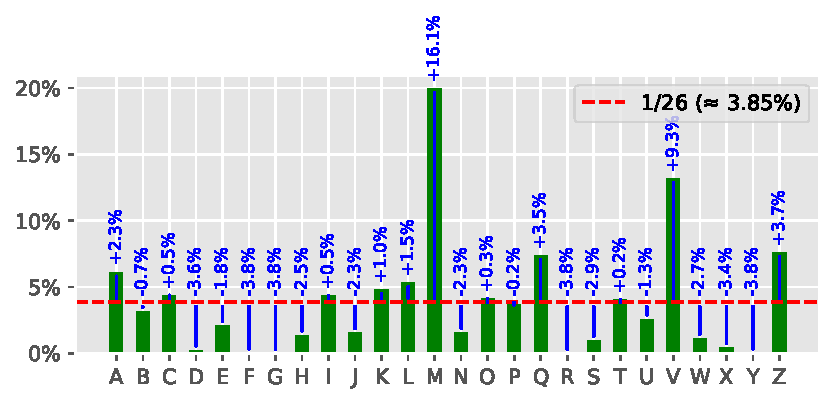
\includegraphics[width=.8\linewidth]{Grundlagen_Info/03_Kryptologie/Figures/vigenere-len3-group1-avg}
	\caption{Buchstabenhäufigkeit in einem mit Caesar verschlüsselten Text, im Vergleich zur Gleichverteilung von Buchstaben}
	\label{fig:vig-subgroup-1-avg}
\end{figure}

Je grösser die blauen Pfeile in \cref{fig:vig-subgroup-1-avg}, desto höher die Friedmansche Charakteristik.

Wir können nun folgenden \emph{Brute-Force}-Ansatz verwenden, um die Schlüssellänge mit der Friedmanschen Charakteristik zu bestimmen:

\begin{itemize}
	\item Alle möglichen Schlüsselwortlängen von 1 bis zu einer beliebig gewählten Zahl $n$ ausprobieren, wobei $n$ praktisch nie über 10 gewählt wird.
	\item Buchstaben jeweils in Gruppen unterteilen:
	      \begin{itemize}
		      \item \textbf{2 Gruppen}: \texttt{\colorstring[ForestGreen,RoyalBlue]{MUZ KJL QPA WJU MHY IIL LCZ AUP MRL ZHL SVC
				            MTZ BCU LGU PCI MPD QGT IPC QIL VGY MGU BUJ
				            PNB MUZ MNA PGY HNP KJL OTH BWS IVP WPK IHB}}
		            \begin{figure}[H]
			            \centering
			            \foreach \i/\groupColor in {1/ForestGreen,2/RoyalBlue} {
					            \begin{subfigure}{.24\textwidth}
						            \centering
						            \includegraphics[width=\textwidth]{Grundlagen_Info/03_Kryptologie/Figures/vigenere-len2-group\i}
						            \caption{\textcolor{\groupColor}{Gruppe \i}}
					            \end{subfigure}}
			            \caption{Buchstaben-Häufigkeiten und $FC_T$ für Schlüssellänge=2}
		            \end{figure}

		      \item \textbf{3 Gruppen}: \texttt{\colorstring[ForestGreen,RoyalBlue,Crimson]{MUZ KJL QPA WJU MHY IIL LCZ AUP MRL ZHL SVC
				            MTZ BCU LGU PCI MPD QGT IPC QIL VGY MGU BUJ
				            PNB MUZ MNA PGY HNP KJL OTH BWS IVP WPK IHB}}
		            \begin{figure}[H]
			            \centering
			            \foreach \i/\groupColor in {1/ForestGreen,2/RoyalBlue,3/Crimson} {
					            \begin{subfigure}{.24\textwidth}
						            \centering
						            \includegraphics[width=\textwidth]{Grundlagen_Info/03_Kryptologie/Figures/vigenere-len3-group\i}
						            \caption{\textcolor{\groupColor}{Gruppe \i}}
					            \end{subfigure}}
			            \caption{Buchstaben-Häufigkeiten und $FC_T$ für Schlüssellänge=3}
		            \end{figure}
		      \item \textbf{4 Gruppen}: \texttt{\colorstring[ForestGreen,RoyalBlue,Crimson,LightSlateBlue]{MUZ KJL QPA WJU MHY IILLCZ AUP MRL ZHL SVC MTZ BCU LGU PCI MPD QGT IPC QIL VGY MGU BUJ PNB MUZ MNA PGY HNP KJL OTH BWS IVP WPK IHB}}
		            \begin{figure}[H]
			            \centering
			            \foreach \i/\groupColor in {1/ForestGreen,2/RoyalBlue,3/Crimson,4/LightSlateBlue} {
					            \begin{subfigure}{.24\textwidth}
						            \centering
						            \includegraphics[width=\textwidth]{Grundlagen_Info/03_Kryptologie/Figures/vigenere-len4-group\i}
						            \caption{\textcolor{\groupColor}{Gruppe \i}}
					            \end{subfigure}}
			            \caption{Buchstaben-Häufigkeiten und $FC_T$ für Schlüssellänge=4}
		            \end{figure}
		      \item etc, bis zu Schlüssellänge = n
	      \end{itemize}
	\item Für jede der Schlüssellängen: Durchschnittliche $FC(T)$ für alle Gruppen berechnen.
	\item Wenn die richtige Schlüssellänge (oder ein Vielfaches davon) gewählt wurde, sollte $FC(T)$ höher sein.
\end{itemize}

Die durchschnittliche Friedmansche Charakteristik für jede der getesteten Schlüssellängen ist gezeigt in \cref{fig:fc}.

\begin{figure}[H]
	\centering
	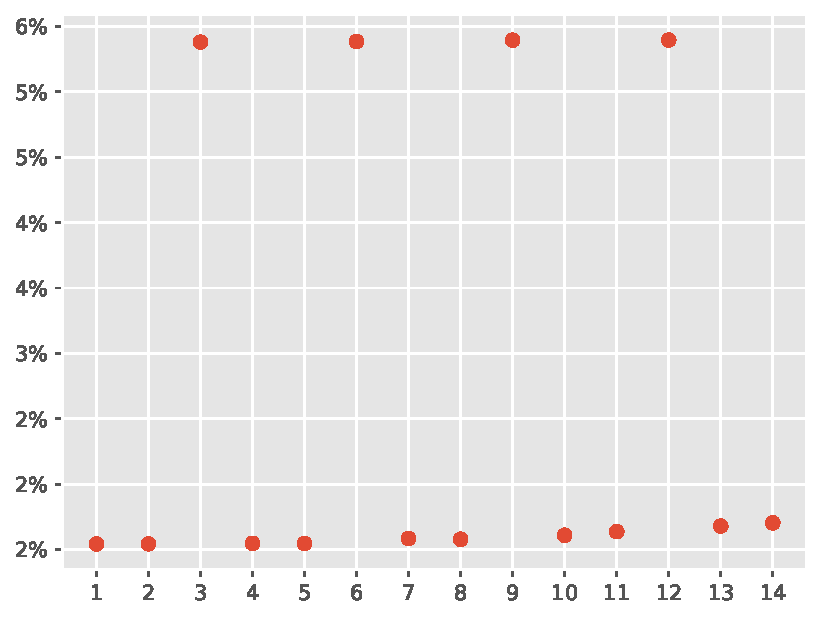
\includegraphics[width=.6\linewidth]{Grundlagen_Info/03_Kryptologie/Figures/friedman}
	\caption{Durchschnittliche Friedmansche Charakteristik für jede Schlüssellänge}
	\label{fig:fc}
\end{figure}

Aus \cref{fig:fc} lässt sich ablesen, dass die Schlüssellänge vermutlich 3 sein muss, da bei jedem Vielfachen der Schlüssellänge 3 die durchschnittliche Friedmansche Charakteristik höher ist als für die restlichen Schlüssellängen. Ab nun lässt sich gleich vorgehen wie in \cref{subsubsec:vigHack} beschrieben, um den Text zu entschlüsseln.

\begin{myexercise}
	Berechnen Sie die Friedmansche Charakteristik für folgende beide Texte von Hand:

	\texttt{\colorstring[black]{PAPPERLAPAPP}}

	\texttt{\colorstring[black]{BACKSTEIN}}

	Wie interpretieren Sie die beiden Zahlen?
	\begin{myanswer}
		Die Friedmansche Charakteristik beträgt 29.5\% und 7.3\%, respektive. Wie Sie sehen, ist die Friedmansche Charakteristik höher für Texte, bei denen jeder Buchstabe relativ häufiger vorkommt.
	\end{myanswer}
\end{myexercise}

\begin{myexercise}
	Für welche Buchstabenverteilung sollte die Friedmansche Charakteristik höher sein: \cref{fig:langer-text-vig-caesar}, (a) oder (b)?
	\begin{myanswer}
		$FC(T)$ sollte für \cref{fig:langer-text-vig-caesar} (a) höher sein, da die durchschnittliche relative Häufigkeit der Buchstaben im Kryptotext ungleicher ist.
	\end{myanswer}
\end{myexercise}


\begin{myexercise}

	Kopieren Sie den folgenden Kryptotext und versuchen Sie, ihn mit dem \href{https://cryptbreaker.marcwidmer.xyz}{Analysetool} zu entziffern, indem Sie zuerst das Tool \emph{Friedman} und danach das Tool \emph{Frequency} verwenden. Wie lautet der Schlüssel?

	\texttt{\colorstring[black]{FZNZKVEDZFCRRZVFZTZFLVIOVBKMZWOVGVBAVSZSMVEDBHVNJANVNBZFZCCRFESPSTJEITSLECZJEGNAPIGZBEZEDQIDIOUBEZZAIVRUSOXEIWFJSZWDYBDBBCLZWOLNYTSVUZAJTHHSJEENZFSEIGJEDDSTVRBSHVNYRJVFPSSJOGQIVSZSMVNBSTTHVTGVNDGUNIZRJVMZWOVIXVCZNNCHCUZQLCIXVNVIIPFJTZFTFGVBAZNYSNXEAIFYLZJPERPVJXEHRBJEDBWVRNIOBEIRBJSHSJEEFIOJTYOSLNOSSCEDRFKIXVLFEIBUVJZHAKNDQIKZZWDYNZBOZCCHFZNZBTKRDQILNYPJENDSFZNBFPVSNSSVRHOMVRBSXVSZBBCSDBEZENSORUBSOSLDQLVNRSOEDVGMZEWSURLPANZCCRBDPAHVEDYWFYOCSTFNISBEDZFPSEMTMREXVFUEMIOUUMQIURDBHCIXVFEFDBTKEMBJJMZWOVSROMUENFVYTPBEEUMSJEZZZOVSOFBYLZBTZCCWOUANWOEEMSIVIGWHKUHGUVHGSOZCCRBENDAIFHZBHIANSBDFVZMVNYSOSAXVFCIZUFLNYBBVHZFBEDZFFIDZHBLSZBEDAIBJXFVZUZGZUSRENQIVNHWSDEMYXLEMRJXWZFEVNRSOEIXVERSRWNDEGBEVRFZFZNZBXVLONXZSXVFEHVZNVNYWFLNUOFYLDUFEUISSXRPSOULDQIVNBSTKAGHFEDZFXLEMADYEIRFIMPSDBCCSOEAZVFIAIAFZNZAIVRUSOWUZVMVUIRGLECZFUIZUFXEIKBITYSTRLGABVCCHJXEIRFIUIGORCCGFZNZACZLYSTTHPTERSRSIVNYSTRLGWFSEIRFEDZFVESDBFNIBSSNOIBFJCCKFSEIRUIAZUULNYSSYAZZUDEDBGIEPBENEIBTUAIBVDMZWOVAPUFEDVSNDEMHVEDYWFNEGHVDMDQIYEMIOUDZFIZMHSMXAINJEMZWOVRNSFCEMIIEWDSEZEBSTKAGHFZNZFHVLDSCKEIRBENNSIEEDQIDIXVPWTPBEUEIYFRCCYPVNIHFJTYIERSRWFUEMOVJDMIFTKZBLFEIBUVSORVUEHDBGIZFFUANSJEHVIDYEIKBJSJJPCLNCXRRHWOUIMZFSTYOTJENKVVRYSEVRNDJVGZZEVIISSJEZZFNIZRFZNZGFVLZWTKDZFTGIZUFCDZGVEEIRMZCCSOXOOHFJMZWOWRZIOUAWSSZCCUFYEYOSLEWSSQUBFVEDZWDYEMZJVGZIOKEMRFIGZKBCTYSSYEMFMZCCYFZTYWFJEMSSJCCSJEUIUFEEDBFNUIRFIBVFFYEDHFIKZWUYAOAFZNZUBEZZGFVLZSJEGZBPDMZBHCEDQIUEIGVVSNSOWRPSICIIUTDOMUFEDDSJTHHWUXAINFDHZFAVNBSOZENGFZCCPJEAGZFZNPBEWRZIFDIXVNVIISTCEWSOJIIRJVSZFHVGZBEUIZTVVRNCMTHZGFVLZBHVSXVBWFZBJJTRWFUIZAFZNZWDYBDBTFGGIFTKGWDYMZWOSENHFISJU}}

	\begin{myanswer}
		Der Schlüssel lautet \texttt{BRAVO}.
	\end{myanswer}
\end{myexercise}

\begin{mychallenge}
	Berechnen Sie die Friedmansche Charakteristik für folgenden Kryptotext:

	\texttt{\colorstring[black]{WORBHHHLUQOWWLDSYSQOWOUKSUDSNEGAAZAEBKISMRILHGPCVLIBZTRLMHYUSIEBILWJKULZSPGHCEFZUQOIQOWCOLSBCVKISZMOSFSZTNBHOSTSUFILHZPCVTEWUHSYZBVCVQEBLMKHHBNEBLIUAIVYDFHEBNTSBCVGUBBNUBTGVMCLGHPHFDAZAEBDISPHFHUGKUBZTIUDBLBSSUATIQOSHLIUAMSPNPBS}}

	Verwenden Sie dazu das Python-Skript auf Moodle, mit der Funktion \lstinline|def calculate_fc(text)|. Was entnehmen Sie aus Ihrer Antwort? Wurde der Text mit Caesar oder mit Vigenère verschlüsselt?

	\begin{myanswer}
		Der tiefe Wert von 1.4\% deutet darauf hin, dass der Text vermutlich mit Vigenère verschlüsselt wurde.
	\end{myanswer}
\end{mychallenge}

\begin{mychallenge}[Ver- und Entschlüsselung mit Python (zu zweit)]
	Laden Sie zuerst die Vigenère-Python-Dateien von Moodle herunter. Erstellen Sie danach einen Text in deutscher Sprache mit mindestens 1000 Zeichen, beispielsweise mittels folgender Webseite: \url{https://www.blindtextgenerator.de/}. Diesen werden Sie nun mit Python verschlüsseln.

	Teil 1: Verschlüsselung
	\begin{itemize}
		\item Verschlüsseln Sie Ihren Text, indem Sie die Funktion \lstinline|def vigenere(text, key, encrypt=True)| verwenden.
		\item Senden Sie Ihren verschlüsselten Text an Ihre(n) Partner(in), nicht aber den Schlüssel.
	\end{itemize}
	Teil 2: Entschlüsselung
	\begin{itemize}
		\item Sie erhalten den Kryptotext und müssen nun zuerst den Schlüssel herausfinden. Bestimmen Sie diesen mithilfe der Friedmanschen Charakteristik, indem Sie die Funktion \lstinline|def get_friedman_vals(text, maxkeylen)| verwenden.
		\item Nachdem Sie die Schlüssellänge bestimmt haben, finden Sie innerhalb jeder Gruppe dem häufigsten Buchstaben. Dies können Sie mit der Funktion \lstinline|def show_letter_freq(text)| einfach umsetzen. Somit sollten Sie das Schlüsselwort herausfinden können.
		\item Entschlüsseln Sie nun den Kryptotext, indem Sie die Funktion \lstinline|def vigenere(text, key, encrypt=False)| verwenden.
	\end{itemize}

\end{mychallenge}

\begin{mychallenge}
	Lösen Sie drei \emph{beliebige Probleme} auf der \href{https://cryptbreaker.marcwidmer.xyz}{Analyse-Webseite}.
\end{mychallenge}


\section{\texorpdfstring{\acrlong{OTP}}{OTP}}

Der Fortschritt in der Mathematik und das neu dazugekommene Wissen machten Vigenère zu einem unsicheren Kryptosystem.

Vigenère und dessen Kryptoanalyse haben wir bereits besprochen. Wir haben gesehen, dass eine Kryptoanalyse vor allem dann leicht ist, wenn der verwendete Schlüssel zu kurz gewählt wird, denn die wesentliche Schwäche von Vigenère ist die Wiederholung der Muster im Kryptotext bei zu kurz gewähltem Schlüssel. Betrachten wir als Beispiel einen Kryptotext aus 1000 Buchstaben, der mit einem Schlüssel der Länge fünf verschlüsselt ist. Das bedeutet, dass jeder fünfte Buchstabe und somit insgesamt je 200 Buchstaben anhand der gleichen Zeile der Vigenère-Tabelle verschlüsselt sind. Das heisst, dass je 200 Buchstaben mit dem gleichen Schlüsselbuchstaben verschlüsselt sind. Durch eine Häufigkeitsanalyse von 200 Buchstaben kann ein Kryptoanalytiker bereits den entsprechenden Buchstaben des Schlüssels bestimmen. Was wäre aber, wenn der verwendete Schlüssel aus 50 Buchstaben bestehen würde? Dann muss eine Häufigkeitsanalyse von 50 Teilen zu je 20 Buchstaben gemacht werden. Es ist nicht garantiert, dass man aus nur 20 Buchstaben eine repräsentative Häufigkeitsverteilung erhält. Gehen wir noch einen Schritt weiter und wählen einen Schlüssel, der genau gleich lang ist wie der Klartext. Nun ist eine Häufigkeitsanalyse völlig unmöglich, da wir es mit 1000 Teilen zu je nur einem Buchstaben zu tun haben.

Die One-Time-Pad-Verschlüsselungsmethode (\gls{OTP}, deutsch \emph{Einmalschlüssel-Verfahren}) funktioniert im Prinzip identisch wie die Vigenère-Methode, mit folgenden drei Unterschieden:
\begin{enumerate}
	\item Der Schlüssel besteht aus einer \emph{zufälligen} Folge von Buchstaben
	\item Der Schlüssel ist \emph{genau gleich lang} wie der Klartext/Kryptotext
	\item Der Schlüssel wird nur für genau eine Botschaft verwendet
\end{enumerate}

\begin{myexample}
Folgendes Beispiel verwendet einen \gls{OTP}-Schlüssel:

\begin{verbatim}
  Klartext: OERLIKON
 Schlüssel: IGBQPWXD
Kryptotext: WKSBXGLQ
\end{verbatim}
\end{myexample}

Essentiell handelt es sich beim \gls{OTP} um dasselbe Verschlüsselungsverfahren wie bei Vigenère, wobei der Schlüssel gleich lang wie die zu verschlüsselnde Nachricht sein muss. Diese Methode gilt als sicher, da die gruppenweise Häufigkeitsanalyse (z.B. mit der Friedmanschen Charakteristik) nicht funktioniert. Allerdings ist die \gls{OTP}-Methode aufgrund der längeren Schlüssellänge mit höheren Übertragungskosten verbunden. Zudem darf jeder Schlüssel zur Sicherheit nur einmal verwendet werden, was für regelmässige Datenaustausch-Anwendungen wie E-Mail, Online-Banking etc. unpraktisch ist.

\begin{myprocedure}[Kryptosystem \gls{OTP}]\label{myprocedure:onetime}
	\leavevmode
	\begin{description}
		\item[Klartextalphabet:] Alphabet der lateinischen Grossbuchstaben.
		\item[Kryptotextalphabet:] Alphabet der lateinischen Grossbuchstaben.
		\item[Schlüsselmenge:] Alle denkbaren Texte bestehend aus lateinischen Grossbuchstaben, welche dieselbe Länge haben wie der Klartext. Es ist wichtig, dass für jeden Klartext ein Schlüssel zufällig generiert wird.
		\item[Verschlüsselung:] Gegeben ist ein zufällig gewählter Schlüssel $s$ aus der Schlüsselmenge. Der gegebene Klartext wird nun (wie gewohnt) mit Hilfe der Vigenère-Tabelle mit dem Schlüssel $s$ verschlüsselt. Der Schlüssel darf danach nicht mehr verwendet werden.
		\item[Entschlüsselung:] Gegeben ist ein zufällig gewählter Schlüssel $s$ aus der Schlüsselmenge. Der gegebene Kryptotext wird (wie gewohnt) durch Vigenère mit dem Schlüssel $s$ entschlüsselt.
	\end{description}
\end{myprocedure}

Warum erscheint uns das \gls{OTP} als ein sicheres Kryptosystem? Die Intuition ist wie folgt. Weil der Schlüssel zufällig gewählt wird und genauso lang ist wie der Klartext, wird jeder Buchstabe des Klartextes um zufällig viele Positionen im Alphabet verschoben. Damit kann man den Kryptotext als eine zufällige Folge von Buchstaben betrachten. Und aus einer zufälligen Folge von Buchstaben kann man keine Informationen herauslesen.

Alice und Bob haben sich in einem geheimen Treffen schon vor einigen Tagen auf den geheimen Schlüssel der Länge 5 für das \gls{OTP} geeinigt. Alice verwendet nun den mit Bob vereinbarten Schlüssel, um eine geheime Nachricht (Kryptotext) an ihn zu senden. Der gesendete Kryptotext lautet \verb|GVRCL|.

Eve hat den Nachrichtenaustausch belauscht und somit den Kryptotext in Erfahrung
gebracht. Sie möchte nun den Klartext herausfinden um zu erfahren, was Alice und Bob unternehmen werden. Eve vermutet, dass der Kryptotext mit dem sicheren \gls{OTP} verschlüsselt ist. Da der verwendete Schlüssel gleich lang ist wie der Klartext, ist eine Kryptoanalyse mit der Häufigkeitsanalyse unmöglich.

\begin{myexercise}
	\begin{aenum}
		\item Wie viele mögliche Schlüssel der Länge 5 gibt es?
		\item Kann Eve den Kryptotext \verb|GVRCL| entschlüsseln, falls sie (im schlimmsten Fall) alle Möglichkeiten durchprobiert?
	\end{aenum}
	\begin{myanswer}
		\begin{aenum}
			\item Es gibt $26^5 = 11'881'376$ verschiedene Möglichkeiten.
			\item Selbst wenn sie alle Schlüssel ausprobieren würde, gäbe es viele Klartexte die denkbar wären. Eve könnte nicht wissen, welches der tatsächliche Klartext ist.
		\end{aenum}
	\end{myanswer}
\end{myexercise}
Dennoch hat Eve das Gefühl, dass sie die geheime Nachricht erraten kann. Die Anzahl aller Klartexte, die aus fünf Buchstaben einen sinnvollen Text ergeben, wird vermutlich nicht so gross sein. Ausserdem weiss Eve, dass sich Alice und Bob verabreden wollen. Eve listet deshalb einige sinnvolle Texte zu je fünf Buchstaben auf. Für jeden dieser möglichen Klartexte bestimmt sie den Schlüssel (mit Hilfe der Vigenère-Tabelle), der den entsprechenden Text zu dem
gegebenen Kryptotext \verb|GVRCL| verschlüsseln würde.

\begin{table}[H]
	\centering
	\begin{tabular}{c|c}
		möglicher Klartext & entsprechender Schlüssel \\ \midrule\midrule
		BADEN              & FVOYY                    \\\midrule
		ESSEN              & CDZYY                    \\\midrule
		LESEN              & VRZYY                    \\\midrule
		SPORT              & OGDLS                    \\\midrule
		VIDEO              & LNOYX
	\end{tabular}
	\caption{Entsprechende Schlüssel bei geratenen möglichen Klartexten (BADEN, ESSEN, LESEN, SPORT, VIDEO) für abgehörten Kryptotext GVRCL.}
	\label{tab:GVRCL}
\end{table}

Jeder dieser Texte kann also durch den angegebenen Schlüssel zum Kryptotext \verb|GVRCL| verschlüsselt werden. Welcher Text entspricht nun der richtigen Nachricht? Alice und Bob haben ihren geheimen Schlüssel zufällig bestimmt, das heisst, jeder mögliche Schlüssel kann mit der gleichen Wahrscheinlichkeit ausgewählt werden. Eve hat daher keine Möglichkeit herauszufinden, welche dieser fünf möglichen Klartexte der geheimen Nachricht entspricht. Es ist auch möglich, dass der richtige Klartext nicht in der Liste steht. Somit hat Eve keine Chance irgendeinen Teil des Klartextes oder des Schlüssels zu erfahren.

Ein Hauptproblem aller symmetrischen Verschlüsselungsverfahren besteht jedoch darin, dass der Schlüssel erst einmal über einen \emph{sicheren} Kanal ausgetauscht werden muss. Vor dem Internet erfolgte dies durch einen Postboten, heute ist dies allerdings nicht mehr praktikabel. Dies werden wir im nächsten Kapitel besprechen.

\begin{myexercise}
	Wie viele mögliche Schlüssel hat der \gls{OTP} für eine Nachricht der Länge $n$?
	\begin{myanswer}
		$26^n$.
	\end{myanswer}
\end{myexercise}

\subsection{Kryptoanalyse bei mehrfacher Verwendung des Schlüssels}

Nun wollen wir wissen, weshalb ein Schlüssel beim \gls{OTP} nur einmal verwendet werden darf. Dazu schauen wir uns einen erneuten Nachrichtenaustausch zwischen Alice und Bob an. Alice möchte Bob nämlich eine weitere geheime Nachricht schicken. Da die zwei jedoch zuvor keinen zweiten Schlüssel vereinbart haben, verwendet Alice den gleichen Schlüssel ein zweites Mal. Diesmal erhält Bob von Alice den folgenden Kryptotext: \verb|ADRCM|.

Eve hat ihr Vorhaben, die beiden zu belauschen, noch nicht aufgegeben und versucht erneut die verschlüsselte Mitteilung zu lesen. Wenn Alice und Bob für die zweite Nachricht einen neuen zufälligen Schlüssel ausgemacht hätten, dann könnte Eve erneut nichts mit dem Kryptotext anfangen. Alice war jedoch nachlässig und verwendete den gleichen Schlüssel ein zweites Mal, um sich mit Bob zu verabreden. Eve ergänzt ihre Tabelle mit einer dritten Spalte. In dieser Spalte notiert sie den Klartext, der entsteht, wenn sie den zweiten Kryptotext mit dem entsprechenden Schlüssel aus der zweiten Spalte entschlüsselt.
\begin{table}[H]
	\centering
	\begin{tabular}{c|c|c}
		möglicher Klartext & entsprechender Schlüssel     & möglicher Klartext für die zweite Nachricht \\ \midrule
		BADEN              & \textcolor{DarkGreen}{FVOYY} & \textcolor{Red}{VIDEO}                      \\
		ESSEN              & CDZYY                        & YASEO                                       \\
		LESEN              & VRZYY                        & FMSEO                                       \\
		SPORT              & OGDLS                        & FMSEO                                       \\
		VIDEO              & LNOYX                        & PQDEP
	\end{tabular}
	\caption{Entschlüsselung eines weiteren abgehörten Kryptotextes (ADRCM) durch die vorher bestimmten denkbaren Schlüsselkandidaten. Der Schlüsselkandidat FVOYY erzeugt aus beiden abgehörten Kryptotexten einen sinnvollen Klartext.}
	\label{tab:ADRCM}
\end{table}
\noindent
Und siehe da, fast alle Texte in der dritten Spalte ergeben keinen Sinn, ausser dem Text
in der ersten Zeile. Eve erkennt, dass mit dem Schlüssel FVOYY sowohl der erste wie auch
der zweite Kryptotext zu einem sinnvollen Text entschlüsselt werden können. Durch den
Vergleich der Entschlüsselungen des ersten und des zweiten Kryptotextes bei gleichem
Schlüssel konnte Eve die tatsächlichen Klartexte und den Schlüssel herausfinden.

\clearpage
\subsection{\texorpdfstring{Bin-\gls{OTP}}{Bin-OTP}}
Das Kryptosystem Bin-\gls{OTP} funktioniert fast gleich wie das \gls{OTP}, nur dass wir nicht mit dem lateinischen Alphabet der Grossbuchstaben arbeiten wollen, sondern lediglich mit dem binären Alphabet $\lrc{0,1}$. Aus der grossen Vigenère-Tabelle in \cref{tab:vigenere} wird im binären Alphabet die übersichtliche (binäre) Vigenère-Tabelle:
\begin{figure}[H]
	\centering
	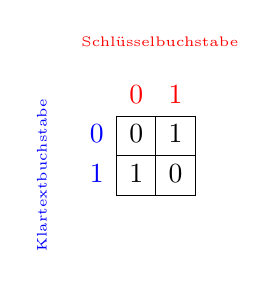
\begin{tikzpicture}
		\foreach \i in {0,...,1} {
				\node at (-0.5,-\i*0.5) {\textcolor{Blue}{\strut \i}};
				\node at (\i*0.5,0.5) {\textcolor{Red}{\strut \i}};
				\foreach \j in {0,...,1} {
						\edef\k{\ifnum\numexpr\i+\j\relax>1
								\the\numexpr\i+\j-2\relax
							\else
								\the\numexpr\i+\j\relax
							\fi}
						\node[draw,minimum size=0.5cm,inner sep=0pt]
						at (\i*0.5,-\j*0.5) {\strut\k};
					}
			}

		\node at (0.3,1.2) {\tiny{\textcolor{Red}{Schlüsselbuchstabe}}};
		\node[rotate = 90] at (-1.2,-0.5)  {\tiny{\textcolor{Blue}{Klartextbuchstabe}}};
	\end{tikzpicture}
	\caption{Vigenère-Tabelle für das binäre Alphabet.}
	\label{fig:VigenereBin}
\end{figure}
\noindent
Der Tabelle entnehmen wir, dass der Klartextbuchstabe $0$ durch den Schlüssel $0$ zum Kryptotextbuchstaben $0$ wird. Man verwendet für die Verschlüsselung mit der binären Vigenère-Tabelle eine besondere Schreibweise. Für die Verschlüsselung des Klartextbuchstaben $0$ durch den Schlüssel $0$ schreiben wir
\begin{align*}
	0 \oplus 0 = 0.
\end{align*}
Wird 0 durch 1 verschlüsselt erhalten wir den Kryptotextbuchstaben 1 (siehe Tabelle) und schreiben
\begin{align*}
	0 \oplus 1 = 1.
\end{align*}
Bitte beachten Sie, dass auch
\begin{align*}
	1 \oplus 0 = 1
\end{align*}
sowie
\begin{align*}
	1 \oplus 1 = 0
\end{align*}
gilt.
\noindent
Die Verschlüsselung mit dem binären \gls{OTP} erfolgt nun, indem Bit für Bit die Operation $\oplus$ (gemäss binärer Vigenère-Tabelle) durchgeführt wird. Analog haben wir mit den lateinischen Buchstaben auch die Verschlüsselung Buchstabe für Buchstabe mithilfe der Vigenère-Tabelle durchgeführt.

\begin{myexample}Folgendes Beispiel illustriert, wie die Verschlüsselung mit dem Bin-\gls{OTP} funktioniert:
\begin{itemize}
	\item
	      Der Klartext ist gegeben durch $\textcolor{Blue}{101}$ und der Schlüssel durch $\textcolor{DarkGreen}{111}$. Dann ist der Kryptotext gegeben durch
	      $\textcolor{Blue}{101} \oplus \textcolor{DarkGreen}{111} = \textcolor{Red}{010}$:
	      \begin{center}
		      \begin{tabular}{cccc}
			             & \textcolor{Blue}{1}      & \textcolor{Blue}{0}      & \textcolor{Blue}{1}      \\
			      \oplus & \textcolor{DarkGreen}{1} & \textcolor{DarkGreen}{1} & \textcolor{DarkGreen}{1} \\
			      \hline
			             & \textcolor{Red}{0}       & \textcolor{Red}{1}       & \textcolor{Red}{0}
		      \end{tabular}
	      \end{center}
	\item
	      Der Klartext ist gegeben durch $\textcolor{Blue}{011101}$ und der Schlüssel durch $\textcolor{Red}{110001}$. Dann ist der Kryptotext gegeben durch
	      \begin{align*}
		      \textcolor{Blue}{011101} \oplus \textcolor{DarkGreen}{110001} = \textcolor{Red}{101100}.
	      \end{align*}
\end{itemize}
\end{myexample}

\begin{myexercise}
	Berechnen Sie den Kryptotext zu dem gegebenen Klartext
	\begin{align*}
		110010100
	\end{align*}
	und zum Schlüssel
	\begin{align*}
		101110001.
	\end{align*}
	\begin{myanswer}
		Der Kryptotext lautet
		\[
			\begin{array}{r}
				110010100         \\
				\oplus\;101110001 \\
				\hline
				011100101
			\end{array}
		\].
	\end{myanswer}
\end{myexercise}

\begin{myexercise}
	\begin{aenum}
		\item Berechnen Sie sowohl
		\begin{align*}
			\textcolor{Red}{100110}\oplus \textcolor{Blue}{001011}
		\end{align*}
		als auch
		\begin{align*}
			\textcolor{Blue}{001011}\oplus \textcolor{Red}{100110}.
		\end{align*}
		Was stellen Sie fest?
		\item Seien $a$ und $b$ zwei beliebige Bits. Begründen Sie, warum stets die Gleichheit
		\begin{align*}
			a\oplus b = b\oplus a
		\end{align*}
		gilt. Wie heisst diese Eigenschaft?
	\end{aenum}
	\begin{myanswer}
		\begin{aenum}
			\item Wir berechnen
			\begin{align*}
				\textcolor{Red}{100110}\oplus \textcolor{Blue}{001011} = \textcolor{DarkGreen}{101101}
			\end{align*}
			sowie
			\begin{align*}
				\textcolor{Blue}{001011}\oplus \textcolor{Red}{100110} = \textcolor{DarkGreen}{101101}.
			\end{align*}
			In beiden Fällen erhalten wir dasselbe Resultat.
			\item Es gibt lediglich die 4 Fälle, welche wir der binären Vigenère-Tabelle entnehmen können. In den beiden Fällen $a = b = 0$ sowie $a = b = 1$ ist die Reihenfolge von $a$ und $b$ offensichtlich jeweils irrelevant, da sie identisch sind. In den beiden Fälle $a = 1$ und $b = 0$ sowie $a = 0$ und $b =1$ gilt
			\begin{align*}
				a\oplus b = 1\oplus 0 = 1 = 0\oplus 1 = b\oplus a.
			\end{align*}
			Damit sagt man, dass die Operation $\oplus$ \emph{kommutativ} ist. Die Reihenfolge der Operanden spielt bei der Operation $\oplus$ keine Rolle.
		\end{aenum}
	\end{myanswer}
\end{myexercise}

\begin{myexercise}
	Sei $a$ eine beliebige binäre Folge (denken Sie sich z.B. $a = 1100101$).
	\begin{aenum}
		\item Was macht die Verschlüsselung $a\oplus a$ von $a$ mit sich selbst?
		\item Mit $0$ bezeichnen wir im Folgenden eine Folge aus lauter Nullen derselben Länge wie $a$. Was macht die Operation $a\oplus 0$?
	\end{aenum}
	\begin{myanswer}
		Mit Hilfe der binären Vigenère-Tabelle begründen wir:
		\begin{aenum}
			\item $a\oplus a = 0$
			\item $a\oplus 0 = a$
		\end{aenum}
	\end{myanswer}
\end{myexercise}
Es lässt sich beweisen, dass die Operation $\oplus$ auch \emph{assoziativ} ist. Die Klammerung der Terme spielt also keine Rolle. Für beliebige binäre Folgen $a,b$ und $c$ derselben Länge gilt also
\begin{align*}
	(a\oplus b) \oplus c = a\oplus (b\oplus c).
\end{align*}
Dies gilt auch für mehr als drei Operanden.

\begin{myexercise}
	Es sei $t$ ein gegebener (binärer) Klartext. Alice wählt zufällig einen binären Schlüssel $s_A$ derselben Länge wie $t$ und berechnet
	\begin{align*}
		k_A := t\oplus s_A.
	\end{align*}
	Was erhält Alice, wenn sie nun
	\begin{align*}
		k_A\oplus s_A
	\end{align*}
	berechnet, also ihren Schlüssel erneut anwendet?
	\begin{myanswer}
		Sie erhält den Klartext $t$ zurück, denn
		\begin{align*}
			k_A\oplus s_A & =                                          \\
			              & (t\oplus s_A)\oplus s_A =                  \\
			              & t\oplus (s_A\oplus s_A) =                  \\
			              & t\oplus \underbrace{s_A\oplus s_A}_{= 0} = \\
			              & t\oplus 0 =                                \\
			              & t.
		\end{align*}
	\end{myanswer}
\end{myexercise}